\documentclass[a4paper]{article}

\setlength{\parindent}{0pt}
\setlength{\parskip}{1em}

\pagestyle{headings}

\usepackage{amssymb}
\usepackage{amsmath}
\usepackage{amsthm}
\usepackage{mathtools}
\usepackage{graphicx}
\usepackage{hyperref}
\usepackage{color}
\usepackage{microtype}
\usepackage{tikz}
\usepackage{pgfplots}
\usepackage{pgfplotstable}

\newcommand{\N}{\mathbb{N}}
\newcommand{\Q}{\mathbb{Q}}
\newcommand{\Z}{\mathbb{Z}}
\newcommand{\R}{\mathbb{R}}
\newcommand{\C}{\mathbb{C}}
\newcommand{\D}{\mathcal{D}}
\renewcommand{\S}{\mathcal{S}}
\renewcommand{\P}{\mathbb{P}}
\newcommand{\F}{\mathbb{F}}
\newcommand{\E}{\mathbb{E}}
\newcommand{\bra}{\langle}
\newcommand{\ket}{\rangle}


\graphicspath{{Image/}}

\hypersetup{
    colorlinks=true,
    linktoc=all,
    linkcolor=blue
}

\theoremstyle{definition}
\newtheorem*{axiom}{Axiom}
\newtheorem*{claim}{Claim}
\newtheorem*{conv}{Convention}
\newtheorem*{coro}{Corollary}
\newtheorem*{defi}{Definition}
\newtheorem*{eg}{Example}
\newtheorem*{lemma}{Lemma}
\newtheorem*{notation}{Notation}
\newtheorem*{prob}{Problem}
\newtheorem*{post}{Postulate}
\newtheorem*{prop}{Proposition}
\newtheorem*{rem}{Remark}
\newtheorem*{thm}{Theorem}

\DeclareMathOperator{\vdiv}{div}
\DeclareMathOperator{\grad}{grad}
\DeclareMathOperator{\curl}{curl}
\DeclareMathOperator{\Ann}{Ann}
\DeclareMathOperator{\Fit}{Fit}
\DeclareMathOperator{\Diag}{Diag}
\DeclareMathOperator{\tr}{tr}
\DeclareMathOperator{\im}{im}
\DeclareMathOperator{\Mat}{Mat}
\DeclareMathOperator{\Log}{Log}
\DeclareMathOperator{\Isom}{Isom}
\DeclareMathOperator{\Mesh}{Mesh}
\DeclareMathOperator{\Sym}{Sym}
\DeclareMathOperator{\Aut}{Aut}
\DeclareMathOperator{\cosech}{cosech}
\DeclareMathOperator{\Card}{Card}
\DeclareMathOperator{\Gal}{Gal}


\setcounter{section}{-1}

\begin{document}

\title{Category Theory}

\maketitle

\newpage

\tableofcontents

\newpage

\section{Introduction}
I didn't go to the first 3 lectures, so no intro -- sorry. I have no idea on what this course is about, let's see

\newpage

\section{Definitions and examples}
\begin{defi} (1.1)\\
    A category $\mathcal{C}$ consists of:\\
    (a) a collection $\ob\mathcal{C}$ of \emph{objects} $A,B,C$;\\
    (b) a collection $\mor\mathcal{C}$ of \emph{morphisms} $f,g,h$;\\
    (c) two operations domain, codomain assigining to each $f \in \mor\mathcal{C}$ a pair of objects, its \emph{domain} and \emph{codomain}; we write $A \xrightarrow{f} B$ to mean \emph{$f$ is a morphism and $\dom f = A, \cod f = B$};\\
    (d) an operation assigning to each $A \in \ob\mathcal{C}$ a morphism $A \xrightarrow{1_A} A$;\\
    (e) a partial binary operation $(f,g) \to fg$ on morphisms, such that $fg$ is defined iff $\dom f = \cod g$, and $\dom(fg) = \dom g$, $\cod(fg) = \cod(f)$ if $fg$ is defined, satisfying:\\
    (f) $f 1_A = f = 1_B f$ for any $A \xrightarrow{f} B$;\\
    (g) $(fg) h = f(gh)$ whenever $fg$ and $gh$ are defined.
\end{defi}

\begin{rem} (1.2)\\
    (a) This definition is independent of any model of set theory. If we're given a particular model of set theory, we call $\mathcal{C}$ \emph{small} if $\ob \mathcal{C}$ and $\mor\mathcal{C}$ are sets.\\
    (b) Some texts say $fg$ means $f$ followed by $g$, i.e. $fg$ is defined iff $\cod f = \dom g$.\\
    (c) Note that a morphism $f$ is an identity iff $fg = g$ and $hf = h$ whenever the composites are defined. So we could formulate the definition entirely in terms of morphisms.
\end{rem}

\begin{eg} (1.3)\\
    (a) The category $\mathbf{Set}$ has all sets as objects, and all functions between sets as morphisms.\\
    Strictly speaking, morphisms $A \to B$ are pairs $(f,B)$ where $f$ is a set-theoretic function. (See part II logic and sets)\\
    (b) The category $\mathbf{Gp}$ has all groups as objects, group homomorphisms as morphisms.\\
    Similarly, $\mathbf{Ring}$ is the category of rings, $\mathbf{Mod_R}$ is the category of $R$-modules.\\
    (c) The category $\mathbf{Top}$ has all topological spaces as objects, and continuous functions as morphisms.\\
    Similarly, $\mathbf{Unif}$ has all uniform spaces and uniformly continuous functions as morphisms, $\mathbf{Mf}$ has all manifolds and smooth maps correspondingly.\\
    (d) The category $\mathbf{Htpy}$ has the same objects as $\mathbf{Top}$, but morphisms are homotopy classess of continuous functions. More generally, given $\mathcal{C}$, we call an equivalence relation $\simeq$ on $\mor \mathcal{C}$ a \emph{congruence} if $f \simeq g \implies \dom f = \dom g$ and $\cod f = \cod g$, and $f \simeq g \implies fh \simeq gh$ and $kf \simeq kg$ whenever the composites are defined. Then we have a category $\mathcal{C} / \simeq$ with the same objects as $\mathcal{C}$, but congruence classes as morphisms instead.\\
    (e) Given $\mathcal{C}$, the \emph{opposite category} $C^{op}$ has the same objects and morphisms as $\mathcal{C}$, but $\dom$ and $\cod$ are interchanged, and $fg$ in $\mathcal{C}^{op}$ is $gf$ in $\mathcal{C}$.\\
    This leads to the \emph{duality principle}: if $P$ is a true statement about categories, so is the statement $P^*$ obtained from $P$ by reversing all arrows.\\
    (f) A small category with one object is a \emph{monoid}, i.e. a semigroup with $1$. In particular, a group is a small cat ($\Cat$) with one object in which every morphism is an isomorphism (i.e. for all $f, \exists g$ s.t. $fg$ and $gf$ are identities).\\
    (g) A \emph{groupoid} is a category in which every morphism is an isomorphism. For example, for a topological space $X$, the \emph{fundamental groupoid} $\pi(x)$ has all points of $X$ as objects, and morphisms $x \to y$ are homotopy classes $rel\{0,1\}$ of paths $u:[0,1] \to X$ with $u(0) = x$, $u(1) = y$ (if you know how to prove that the fundamental group is a group, you can prove that $\pi(x)$ is a groupoid).\\
    (h) A \emph{discrete} cat is one whose only morphism are identities.\\
    A \emph{preorder} is a cat $\mathcal{C}$ in which, for any pair $(A,B)$, $\exists$ at most 1 morphism $A \to B$.\\
    A small preorder is a set equipped with a binary relation which is reflexive and transitive.\\
    In particular, a partially ordered set is a small preorder in which the only isomorphisms are identities.\\
    (i) The category $\mathbf{Rel}$ has the same objects as \emph{set}, but morphisms $A \to B$ are arbitrary relations $R \subseteq A \times B$. Given $R$ and $S \subseteq B\times C$, we define $S \cdot R = \{(a,c) \in A \times C | (\exists b \in B) ((a,b) \in R, (b,c) \in S)\}$.\\
    The identity $1_A:A \to A$ is $\{(a,a) | a \in A\}$.\\
    Similarly, the category $\mathbf{Part}$ are for sets and partial functions (i.e. relations s.t. $(a,b) \in R$ and $(a,b') \in R \implies b = b'$).\\
    (j) Let $K$ be a field. The cateogry $\mathbf{Mat_K}$ has natural numbers as objects, and morphism $n \to p$ are $(p \times n)$ matrices with entries from $K$. Composition is matrix multiplication.\\
    (k) We write $\mathbf{Cat}$ for the category whose objects are all small categories, and whose morphisms are functors between them. (see below for definition of functors)
\end{eg}

\begin{defi} (1.4)\\
    Let $\mathcal{C}$ and $\mathcal{D}$ be categories. A \emph{functor} $F:\mathcal{C} \to \mathcal{D}$ consists of:\\
    (a) a mapping $A \to FA$ from $\ob \mathcal{C}$ to $\ob \mathcal{D}$;\\
    (b) a mapping $f \to Ff$ from $\mor \mathcal{C}$ to $\mor \mathcal{D}$,\\
    such that $\dom(Ff) = F(\dom f)$, $\cod(Ff) = F(\cod f)$, $1_{FA} = F(1_A)$, and $(Ff)(Fg) = F(fg)$ whenever $fg$ is defined.
\end{defi}

\begin{eg} (1.5)\\
    (a) We have \emph{forgetful functors} $U$: $\mathbf{Gp} \to \mathbf{Set}$, $\mathbf{Ring}\to \mathbf{Set}$, $\mathbf{Top} \to \mathbf{Set}$, $\mathbf{Ring} \to \mathbf{AbGp}$ (forget $\times$), $\mathbf{Ring} \to \mathbf{Mon}$ (Category of all monoids) (forget $+$).\\
    (b) Given a set $A$, the free group $FA$ has the property:\\
    Given any group $G$ and any function $A \xrightarrow{f} UG$ (?), there's a unique homomorphism $FA \xrightarrow{\bar{f}} G$ extending $f$. Here $F$ is a functor $\mathbf{Set}\to \mathbf{Gp}$: given $A \xrightarrow{f} B$, we define $Ff$ to be the unique homomorphism extending $A \xrightarrow{f} B \leftrightarrow UFB$. \href{https://math.stackexchange.com/questions/1922113/what-exactly-is-functoriality}{Functoriality} follows from uniqueness given $B \xrightarrow{f} C$. $F(gf)$ and $(Fg)(Ff)$ are both homomorphisms extending $A \xrightarrow{f} B \xrightarrow{g} C \rightarrow UFC$.\\
    (c) Given a set $A$, we write $PA$ for the set of all subsets of $A$.\\
    We can make $P$ into a functor $\mathbf{Set} \to \mathbf{Set}$, given $A \xrightarrow{f} B$, we defined $Pf(A') = \{f(a) | a \in A'\}$ for $A' \subseteq A$.\\
    But we also have a functor $P^* : \mathbf{Set} \to \mathbf{Set}^{op}$ defined on objects by $P$, but $P^* f(B') = \{a \in A | f(a) \in B'\}$ for $B' \subseteq B$.\\
    By a \emph{contravariant} functor $\mathcal{C} \to \mathcal{D}$, we mean a functor $\mathcal{C} \to \mathcal{D}^{op}$ (or $\mathcal{C}^{op} \to \mathcal{D}$). A \emph{covariant} functor is one that doesn't reverse arrows (in $op$ I guess?).\\
    (d) Let $K$ be a field. We have a functor $*:\mathbf{Mod_K} \to \mathbf{Mod_K}^{op}$ defined by $V^* = \{ \text{ linear maps }  V \to K\}$, and if $V \xrightarrow{f} W$, $f^*(\theta:W \to K) = \theta f$.\\
    (e) We have a functor $op: \mathbf{Cat} \to \mathbf{Cat}$, which is the identity on morphisms (note that this is a covariant).\\
    (f) A functor between monoids is a monoid homomorphism.\\
    (g) A functor between posets is an order-preserving map.\\
    (h) Let $G$ be a group. A functor $F \circ G \to \mathbf{Set}$ consists of a set $A=F*$ together with an action of $G$ on $A$, i.e. a \emph{permutation representation} of $G$.\\
    Similarly, a functor $G \to \mathbf{Mod_K}$ is a $K$-linear representation of $G$.\\
    (i) The construction of the fundamental group $\pi(X,X)$ of a space $X$ with basepoint $X$ is a functor $\mathbf{Top}* \to \mathbf{Gp}$ where $\mathbf{Top}*$ is the category of spaces with a chosen basepoint.\\
    Similarly, the fundamental groupoid is a functor $\mathbf{Top} \to \mathbf{Gpd}$, where $\mathbf{Gpd}$ is the category of groupoids and functors between them.
\end{eg}

\begin{defi} (1.6)\\
    Let $\mathcal{C}$ and $\mathcal{D}$ be categories and $F, G: \mathcal{C}\rightrightarrows \mathcal{D}$ (why two arrows?) two functors.\\
    A \emph{natural transformation} $\alpha:F \to G$ consists of an assignment $A \to \alpha_A$ from $\ob \mathcal{C}$ to $\mor \mathcal{D}$ (think about this), such that $\dom_{\alpha_A} = FA$ and $\cod_{\alpha A} = G A$ for all $A$, and for all $A \xrightarrow{f} B$ in $\mathcal{C}$, the square 
    \begin{equation*}
        \begin{aligned}
            &FA &\xrightarrow{Ff} &FB\\
            &\downarrow \alpha_A & &\downarrow \alpha_B\\
            &GA &\xrightarrow{Gf} & GB
        \end{aligned}
    \end{equation*}
    commutes (i.e. $\alpha_B(Ff) = (Gf)_{\alpha A}$).
\end{defi}

(1.3) (l) Given categories $\mathcal{C}$ and $\mathcal{D}$, we write $[\mathcal{C},\mathcal{D}]$ for the category whose objects are functors $\mathcal{C} \to \mathcal{D}$ and whose morphisms are natural transformations.

\begin{eg} (1.7)\\
    (a) Let $K$ be a field, $V$ a vector space over $K$. There is a linear map $\alpha_V : V \to V^{**}$ given by $\alpha_V (v) \theta = \theta(v)$ for $\theta \in V^*$.\\
    This is the $V$-component of a natural transformation $1_{\mathbf{Mod_K}} \to **: \mathbf{Mod_K} \to \mathbf{Mod_K}$.\\
    (b) For any set $A$, we have a mapping $\sigma_A:A \to PA$ sending $a$ to $\{a\}$. If $f:A \to B$, then $Pf\{a\} = \{f(a)\}$. So $\sigma$ is a natural transformation $1_{\mathbf{Set}} \to P$.\\
    (c) Let $F$:$\mathbf{Set} \to \mathbf{Gp}$ be the free group functor (1.5(b)), and $U: \mathbf{Gp} \to \mathbf{Set}$ the forgetful functor. The inclusions $A \to UFA$ form a natural transformation $1_{\mathbf{Set}} \to UF$.\\
    (d) Let $G,H$ be groups and $f,g: G \rightrightarrows H$ be two homomorphisms. A natural transformation $\alpha: f \to g$ corresponds to an element $h=\alpha_*$ of $H$, s.t. $h f(x) \to g(x) h$ for all $x \in G$ or equivalently $f(x) = h^{-1} g(x) h$, i.e. $f$ and $g$ are conjugate group homomorphisms.\\
    (e) Let $A$ and $B$ be two $G$-sets, regarded as functors: $G \rightrightarrows \mathbf{Set}$. A natural transformation $A \to B$ is a function $f$ satisfying $f(g\cdot a) = g \cdot f(a)$ for all $a \in A$, i.e. a $G$-equivariant map.
\end{eg}

\begin{lemma} (1.8)\\
    Let $F,G: \mathcal{C} \rightrightarrows \mathcal{D}$ be two functors, and $\alpha: F \to G$ a natural transformation. Then $\alpha$ is an isomorphism in $[\mathcal{C},\mathcal{D}]$ iff each $\alpha_A$ is an isomorphism in $\mathcal{D}$.
    \begin{proof}
        Forward is trivial. For backward, suppose each $\alpha_A$ has an inverse $\beta_A$. Given $f:A \to B$ in $\mathcal{C}$, we need to show that 
        \begin{equation*}
            \begin{aligned}
                &GA &\xrightarrow{Gf} &GB\\
                &\downarrow \beta_A & &\downarrow \beta_B\\
                &FA &\xrightarrow{Ff} & FB
            \end{aligned}
        \end{equation*}
    \end{proof}
    commutes. But as $\alpha$ is natural, 
    $$(Ff)\beta_A = \beta_B \alpha_B (Ff)\beta_A = \beta_B (Gf) \alpha_A \beta_A = \beta_B (Gf)$$
    So $\beta$ is a natural transformation as well.
\end{lemma}

\begin{defi} (1.9)\\
    Let $\mathcal{C}$ and $\mathcal{D}$ be categories. By an \emph{equivalence} between $\mathcal{C}$ and $\mathcal{D}$, we mean a pair of functors $F:\mathcal{C} \to \mathcal{D}$, $G:\mathcal{D} \to \mathcal{C}$ together with natural isomorphisms $\alpha: 1_\mathcal{C} \to GF$ and $\beta: FG \to 1_\mathcal{D}$.\\
    We write $\mathcal{C} \cong \mathcal{D}$ if $\mathcal{C}$ and $\mathcal{D}$ are equivalent.\\
    We say a property $P$ of categories is a \emph{categorical property} if whenever $\mathcal{C}$ has $P$ and $\mathcal{C} \cong \mathcal{D}$, then $\mathcal{D}$ has $P$.\\
    For example, being a groupoid or a preorder are categorical properties, but being a group or a partial order are not.
\end{defi}

\begin{eg} (1.10)\\
    (a) The category $\mathbf{Part}$ is equivalent to the category $\mathbf{Set}_*$ of pointed sets (and basepoint preserving functions (as morphisms)):\\
    $\bullet$ We define $F:\mathbf{Set}_* \to \mathbf{Part}$ by $F(A,a) = A \setminus \{a\}$, and if $f:(A,a) \to (B,b)$, then $Ff(x) = f(x)$ if $f(x) \neq b$, and undefined otherwise;\\
    $\bullet$ and $G: \mathbf{Part} \to \mathbf{Set}_*$ by $G(A) = A^+ = (A \cup \{A\},A)$, and if $f:A \to B$ is a partial function, we define $Gf:A^+ \to B^+$ by $Gf(x) = f(x)$ if $x \in A$ and $f(x)$ defined, and equals $B$ otherwise.\\
    The composite $FG$ is the identity on $\mathbf{Part}$, but $GF$ is not the identity. However, there is an isomoprhism $(A,a) \to ((A \setminus \{a\})^+,A \setminus\{a\})$ sending $a$ to $A \setminus \{a\}$ and everything else to itself and this is natural.\\
    Note that there can be no isomoprhism from $\mathbf{Set}_*$ to $\mathbf{Part}$, since $\mathbf{Part}$ has a 1-element isomorphism class $\{\phi\}$ but $\mathbf{Set}_*$ doesn't.\\
    (So we see that equivalent categories can be non-isomorphic. According to a \href{https://mathoverflow.net/questions/30032/equivalence-versus-isomorphism-of-categories}{post} on SO, this usually happens when there are multiple copies of the \emph{same} thing in one but not the other. However, we can't generally \emph{discard obsolete copies} in one as that generally requires AC and is not a very useful thing to do anyway -- In short, \emph{identifying isomorphic objects is often an extremely bad idea}.)\\
    (b) The category $\mathbf{fdMod_K}$ of finite-dimensional vector spaces over $K$ is equivalent to $\mathbf{fdMod_K}^{op}$, the functors in both directions are $*$ (the dual operator) and both isomorphisms are the natural transformations of 1.7(a) (double dual).\\
    (c) $\mathbf{fdMod_K}$ is also equivalent to $\mathbf{Mat}_K$ (1.3(j)):\\
    We define $F:\mathbf{Mat_K} \to \mathbf{fdMod_K}$ by $F(n) = K^n$, and $F(A)$ is the linear map represented by $A$ w.r.t. the standard bases of $K^n$ and $K^p$.\\
    To define $G:\mathbf{fdMod_K} \to \mathbf{Mat_K}$, choose a basis for each finite dimensional vector space, and define $G(V) = \dim V$, $G(V \xrightarrow{f} W)$ to be the matrix representing $f$ w.r.t. chosen bases. $GF$ is the identity, provided we choose the standard bases for the spaces $K^n$; $FG \neq 1$, but the chosen bases give isomorphisms $FG(V) = K^{\dim V} \to V$ for each $V$, which form a natural isomorphism.
\end{eg}

---Lecture 4---

\begin{defi} (1.11)\\
    Let $\mathcal{C} \xrightarrow{F} \mathcal{D}$ be a functor.\\
    (a) We say $F$ is \emph{faithful} if, given $f,f' \in \mor \mathcal{C}$ with $\dom f = \dom f'$, $\cod f = \cod f'$, and $Ff = Ff'$, then $f=f'$ (injectivity on morphisms. The name comes more from representation theory);\\
    (b) We say $F$ is \emph{full} if, given $FA \xrightarrow{g} FB$ in $\mathcal{D}$, there exists $A \xrightarrow{f} B$ in $\mathcal{C}$ with $Ff = g$. (this is something like surjectivivity on morphisms, but see below);\\
    (c) We say  $F$ is \emph{essentially surjective} if, for every $B \in \ob \mathcal{D}$, there exists $A \in \ob \mathcal{C}$ and isomorphism $FA \to B$ in $\mathcal{D}$.\\
    We say a subcategory $\mathcal{C}' \subseteq \mathcal{C}$ is full if the inclusion $\mathcal{C}' \to \mathcal{C}$ is a full functor (basically, if the objects are kept, any morphism between them must be kept). For example, $\mathbf{Gp}$ is a full subcategory of $\mathbf{Mon}$ (the category of all monoids), but $\mathbf{Mon}$ is not a full subcategory of the category $\mathbf{SGp}$ of semigroups (consider e.g. the homomorphism that sends everything in $(\Z,\cdot)$ to $(0,\cdot)$ (which is also a semigroup); but this doesn't preserve 1 so is not a morphism in $\mathbf{Mon}$).
\end{defi}

\begin{lemma} (1.12)\\
    Assuming the axiom of choice, a functor $F:\mathcal{C} \to \mathcal{D}$ is part of an equivalence $\mathcal{C} \simeq \mathcal{D}$ if it's full, faithful, and essentially surjective.
    \begin{proof}
        $\Rightarrow$: Suppose given $G,\alpha,\beta$ as in (1.9). Then for each $B \in \ob\mathcal{D}$, $\beta_B$ is an isomorphism $FGB \to B$, so $F$ is essentially surjective.\\
        Given $A \xrightarrow{f} B$ in $\mathcal{C}$, we can recover $f$ from $Ff$ as composite $A \xrightarrow{\alpha_A} GFA \xrightarrow{GFf} GFB \xrightarrow{\alpha_b^{-1}} B$. Hence if $A \xrightarrow{f'}B$ satisfies $Ff = Ff'$, then $f=f'$. So $F$ is faithful;\\
        Lastly, for fullness, given $FA \xrightarrow{g} FB$, define $f$ to be the composite $A \xrightarrow {\alpha_A} GFA \xrightarrow{Gg} GFB \xrightarrow{\alpha_B^{-1}} B$. Then $GFf = \alpha_B f \alpha_A^{-1}$, which by construction is just $Gg$. But $G$ is faithful for the same reason as $f$, so $Ff = g$.

        $\Leftarrow$: (need to find suitable $G,\alpha,\beta$ for $F$.) For each $B \in \ob \mathcal{D}$, choose $GB \in \ob \mathcal{C}$ and an isomorphism $\beta_B : FGB \to B$ in $\mathcal{D}$. Given $B \xrightarrow{g} B'$, define $Gg:GB \to GB'$ to be the unique morphism whose image under $F$ is $FGB \xrightarrow{\beta_B} B \xrightarrow{g} B' \xrightarrow{\beta_{B'}^{-1}} FGB'$.\\
        Uniqueness implies functoriality: given $B' \xrightarrow{g'} B''$, $(Gg')(Gg)$ and $G(g'g)$ have the same image under $F$, so they are equal.\\
        By construction, $\beta$ is a natural transformation $FG \to 1_\mathcal{D}$.\\
        Given $A \in \ob \mathcal{C}$, define $\alpha_A: A \to GFA$ to be the unique morphism whose image under $F$ is $FA \xrightarrow{\beta_{FA}^{-1}} FGFA$. $\alpha_A$ is an isomorphism, since $\beta_{FA}$ also has a unique pre-image under $F$. And $\alpha$ is a natural transformation, since any naturality square for $\alpha$ (the commutative square when we defined natural transformation) is mapped by $F$ to a commutative square, and $F$ is faithful.
    \end{proof}
\end{lemma}

\begin{defi} (1.13) \\
    By a \emph{skeleton} of a category, we mean a full subcategory $\mathcal{C}_0$ containing one object from each isomorphism class. We say $\mathcal{C}$ is \emph{skeletal} if it's a skeleton of itself.\\
    For example, $\mathbf{Mat_K}$ is a skeletal, and the image of $F:\mathbf{Mat_K} \to \mathbf{fdMod_K}$ of 1.10(c) is a skeleton of $\mathbf{fdMod_K}$.\\
    (there are some examples on wikipedia)
\end{defi}

Warning: almost any assertion about skeletons is equivalent to axiom of choice (see q2 on example sheet 1).

\begin{defi} (1.14)\\
    Let $A \xrightarrow{f} B$ be a morphism in $\mathcal{C}$.\\
    (a) We say $f$ is a \emph{monomorphism} (or $f$ is \emph{monic}) if, given any pair $C \stackrel[h]{g}{\rightrightarrows} A$, $fg=fh$ implies $g=h$.\\
    (b) We say $f$ is an \emph{epimorphism} (or \emph{epic}) if it's a monomorphism in $\mathcal{C}^{op}$, i.e. if $gf = hf$ implies $g=h$.\\
    We denote monomorphisms by $A \stackrel{f}{\rightarrowtail} B$, and epimorphisms by $A \stackrel{f}{\twoheadrightarrow} B$.\\
    Any isomorphism is monic and epic: more generally, if $f$ has a left inverse (i.e. $\exists g$ s.t. $gf$ is an identity), then it's monic. We call such monomorphisms \emph{split}.\\
    We say $\mathcal{C}$ is a \emph{balanced} category if any morphism which is both monic and epic is an isomorphism.
\end{defi}

\begin{eg} (1.15)\\
    (a) As usual we consider $\mathbf{Set}$ first. In $\mathbf{Set}$, monomorphisms correspond to injections ($\Leftarrow$ is easy (ok); for $\Rightarrow$, take $C \rightrightarrows 1 = \{*\}$), and epimorphsims correspond to surjections ($\Leftarrow$ is easy; for $\Rightarrow$, use morphisms $B \rightrightarrows 2 = \{0,1\}$). So $\mathbf{Set}$ is balanced.\\
    (b) In $\mathbf{Gp}$, monomorphisms again correspond to injections (for $\Rightarrow$ use homomorphisms $\Z \to A$); epimorphisms again correspond to surjections ($\Rightarrow$ use \href{https://en.wikipedia.org/wiki/Free_product#Generalization:_Free_product_with_amalgamation}{free products with amalgamation} -- this is a non-trivial fact about groups, read more if free). So $\mathbf{Gp}$ is also balanced.\\
    (c) In $\mathbf{Rng}$ (obvious notation), monomorphisms correspond to injections (proof is much like for $\mathbf{Gp}$). However, not all epimorphisms are surjective. For example the inclusion $\Z \to \Q$ is an epimorphism, since if $\Q \stackrel[g]{f}{\rightrightarrows} R$ (any ring) agree on all integers, they agree everywhere. So $\mathbf{Rng}$ is not balanced.\\
    (d) One final example is $\mathbf{Top}$. Again, monomorphisms are injections and epimorphisms are surjections (and vice versa): proof is similar to $\mathbf{Set}$ (check). However, $\mathbf{Top}$ is not balanced since a continuous bijection need not have continuous inverse.
\end{eg}

\newpage

\section{The Yoneda Lemma}

---Lecture 5---
\begin{defi} (2.1)\\
    We say a category $\mathcal{C}$ is \emph{locally small} if, for any two objects $A,B$, the morphisms $A\to B$ in $\mathcal{C}$ form a set $\mathcal{C}(A,B)$.\\
    If we fix $A$ and let $B$ vary, the assignment $B \to \mathcal{C}(A,B)$ becomes a functor $\mathcal{C}(A,-):\mathcal{C} \to \mathbf{Set}$: given $B \xrightarrow{f} C$, $\mathcal{C}(A,f)$ is the mapping $g \to fg$ for all $g \in \mathcal{C}(B,C)$. Similarly, $A \to \mathcal{C}(A,B)$ defines a functor $\mathcal{C}(-,B):\mathcal{C}^{op} \to \mathbf{Set}$ (for $A \xrightarrow{f} C \in \mor \mathcal{C}^{op}$, maps $g \to gf$).
\end{defi}

\begin{lemma} (2.2)\\
    (i) Let $\mathcal{C}$ be a locally small category, $A \in \ob \mathcal{C}$ and $F:\mathcal{C} \to \mathbf{Set}$ a functor. Then natural transformations $\mathcal{C}(A,-) \to F$ are in bijection with elements of $FA$;\\
    (ii) Moreover, this bijection is natural in $A$ and $F$.
    \begin{proof}
        (i) Given $\alpha$:$\mathcal{C}(A,-) \to F$, we define $\Phi(\alpha) = \alpha_A(1_A) \in FA$.\footnote{Note $1_A \in \mathcal{C}(A,A)$, and $\alpha_A \in \mor \mathbf{Set}$ but $\mor \mathbf{Set}$ are just functions between sets, so this makes sense.}\\
        Conversely, given $x \in FA$, we define $\Psi(x): \mathcal{C}(A,-) \to F$ by $\Psi(x)_B (A \xrightarrow{f} B) = (Ff)(x) \in FB$.\footnote{It seems a bit confusing why this is a natural transformation, but looking carefully it basically defines a function between sets, i.e. is in $\mor \mathbf{Set}$.}\\
        $\Psi(x)$ is natural: given $g:B \to C$, we have
        \begin{equation*}
            \begin{aligned}
                \Psi(x)_C \mathcal{C}(A,g) (f) &= \Psi(x)_C (gf) = F(gf)(x),\\
                (Fg) \Psi(x)_B(f) &= (Fg)(Ff)(x) = F(gf)(x)
            \end{aligned}
        \end{equation*}
        Now given $x \in FA$, $\Phi\Psi(x) = \Psi(X)_A (1_A) = F(1_A)(x) = x$; given $\alpha$,
        \begin{equation*}
            \begin{aligned}
                \Psi\Phi(\alpha)_B(f) \Psi(\alpha_A(1_A))_B(f) &= Ff(\alpha_A(1_A))\\
                &= \alpha_B\mathcal{C}(A,f)(1_A) = \alpha_B(f)
            \end{aligned}
        \end{equation*}
        So $\Psi\Phi(\alpha)=\alpha$. So $\Psi\Phi$ and $\Phi\Psi$ are both identities on their respective domain (so we have a bijection).
    \end{proof}
\end{lemma}

\begin{coro} (2.3)\\
    The assignment $A \to \mathcal{C}(A,-)$ defines a full and faithful functor $\mathcal{C}^{op} \to [\mathcal{C},\mathbf{Set}]$.
    \begin{proof}
        Put $F = \mathcal{C}(B,-)$ in 2.2(i): we get a bijection between $\mathcal{C}(B,A)$ and morphisms $\mathcal{C}(A,-) \to \mathcal{C}(B,-)$ in $[\mathcal{C},\mathbf{Set}]$\footnote{Think very carefully about this... Given a morphism in $\mathcal{C}(A,-) \to \mathcal{C}(B,-)$, the above gives us a way to identify it uniquelly with an element in $\mathcal{C}(B,A)$ which is in $\mor \mathcal{C}^{op}$. But that alone is not enough; we also need the above functor to take that morphism \emph{directly} to the original morphism. Luckily this is the case by the proof of 2.2(i), which is also explained in the later half of the sentence above.}. We need to verify this is functorial: but it sends $f:B \to A$ to the natural transformation $g \to gf$. So functoriality follows from associativity.
    \end{proof}
\end{coro}

We call this functor (or the functor $\mathcal{C} \to [\mathcal{C}^{op}, \mathbf{Set}]$ sending $A$ to $\mathcal{C}(-,A)$) the \emph{Yoneda embedding} of $\mathcal{C}$, and denote it by $Y$.

Now let's go back to prove 2.2(ii):
\begin{proof}
    (ii) Suppose for the moment that $\mathcal{C}$ is small, so that $[\mathcal{C},\mathbf{Set}]$ is locally small.\footnote{Elements in $\mor [\mathcal{C},\mathbf{Set}]$ correspond to those in $\mor \mathcal{C}^{op}$ by Yoneda.} Then we have two functors $\mathcal{C} \times [\mathcal{C},\mathbf{Set}] \to \mathbf{Set}$: one sends $(A,F)$ to $FA$, and the other is the composite: $\mathcal{C} \times [\mathcal{C},\mathbf{Set}] \xrightarrow{Y \times 1} [\mathcal{C},\mathbf{Set}]^{op} \times [\mathcal{C},\mathbf{Set}] \xrightarrow{[\mathcal{C},\mathbf{Set}](-;-)} \mathbf{Set}$.\footnote{The second operator maps two functors two the set of natural transformations between them?}\\
    2.2(ii) says that these are naturally isomorphic. We can translate this into an elementary statement, making sense even when $\mathcal{C}$ isn't small. Given $A \xrightarrow{f} B$ and $F \xrightarrow{\alpha}G$, the two ways of producing an element of $GB$ from a natural transformation $\beta:\mathcal{C}(A,-) \to F$ give the same result, namely $$\alpha_B(Ff)\beta_A(1_A) = (Gf)\alpha_A\beta_A(1_A)$$ which is equal to $\alpha_B\beta_B(f)$.
\end{proof}

\begin{defi} (2.4)\\
    We say a functor $F:\mathcal{C} \to \mathbf{Set}$ is \emph{representable} if it's isomorphic to $\mathcal{C}(A,-)$ for some $A$. By a representation of $F$, we mean a pair $(A,x)$ where $x \in FA$ is such that $\Psi(x)$ is an isomorphism.\\
    We also call $x$ a \emph{universal element} of $F$.
\end{defi}

\begin{coro} (2.5)\\
    If $(A,x)$ and $(B,y)$ are both representations of $F$, then there's a unique isomorphism $f:A \to B$ such that $(Ff)(x) = y$.
    \begin{proof}
        Consider the composite $\mathcal{C}(B,-) \xrightarrow{\Psi(y)^{-1}}F \xrightarrow{\Psi(x)} \mathcal{C}(A,-)$. By (2.3) this is of the form $Y(f)$ for a unique isomorphism $f:A \to B$, and the diagram

        \begin{tikzcd}
            \mathcal{C}(B,-) \arrow[rd,"\Psi(y)"'] \arrow[rr,"Y(f)"] & & \mathcal{C}(A,-) \arrow[dl,"\Psi(x)"]\\
            &F &
        \end{tikzcd}

        commutes iff $(Ff)(x) = y$.
    \end{proof}
\end{coro}

\begin{eg} (2.6)\\
    (a) The forgetful functor $\mathbf{Gp} \to \mathbf{Set}$ is representable by $(\Z,1)$, $\mathbf{Rng} \to \mathbf{Set}$ by $(\Z[X],X)$, and $\mathbf{Top} \to \mathbf{Set}$ by $(\{*\},*)$.\\
    (b) The functor $P^*: \mathbf{Set}^{op} \to \mathbf{Set}$ is representable by $(\{0,1\},\{1\})$: this is the bijection between subsets and characteristic functions.\\
    (c) Let $G$ be a group. The unique (up to isomorphism) representable functor $G(*,-): G \to \mathbf{Set}$ is the \emph{Cayley representation} of $G$, i.e. the set $UG$ with $G$ acting by left multiplication.\\
    (d) Let $A$ and $B$ be two objects of a small category $\mathcal{C}$. We have a functor $\mathcal{C}^{op} \to \mathbf{Set}$ sending $C$ to $\mathcal{C}(C,A) \times \mathcal{C}(C,B)$. A representation of this, if it exists, is called a (categorical) \emph{product} of $A$ and $B$, and denoted $(A \times B,(A \times B \xrightarrow{\pi_1} A, A \times B \xrightarrow{\pi_2} B))$.\\
    This pair has the property that, for any pair $(C \xrightarrow{f}A,C\xrightarrow{g}B)$, there's a unique $C \xrightarrow{h} A \times B$ with $\pi_1 h = f$ and $\pi_2 h = g$.\\
    Products exist in many categories of interest: in $\mathbf{Set}$, $\mathbf{Gp}$, $\mathbf{Rng}$, $\mathbf{Top}$,..., they are \emph{just} cartesian products, in posets they are binary meets (see sheet 1 Q1).\\
    Dually, we have the notion of \emph{coproduct} $(A+B,A \xrightarrow{\mu_1} A + B, B \xrightarrow{\mu_2}A+B)$.\\
    These also exist in many categories of interest.\\
    ---Lecture 6---\\
    (f) (Lecturer didn't like (e) so jumped to (f) directly) Let $A \stackrel[g]{f}{\rightrightarrows} B$ be morphisms in locally small category $\mathcal{C}$. We have a functor $F:\mathcal{C}^{op} \to \mathbf{Set}$ defined by 
    \begin{equation*}
        \begin{aligned}
            F(C) = \{h \in \mathcal{C}(C,A) | fh = gh\}
        \end{aligned}
    \end{equation*}
    A representation (see (2.4)) of $F$, if it exists, is called an \emph{equalizer} of $(f,g)$: It consists of an object $E$ and a morphism $E \xrightarrow{e} A$ s.t. $fe=ge$, and every $h$ with $fh=gh$ factors uniquely (see proof of 2.9(i) which gives an insight of what this means) through $e$.\\
    In $\mathbf{Set}$, we take $E = \{x \in A | f(x) = g(x) \}$ and $e=$inclusion. Similar constructions work in $\mathbf{Gp},\mathbf{Rng},\mathbf{Top}$,...\\
    Dually, we have the notion of \emph{coequalizer}.
\end{eg}

\begin{rem} (2.7)\\
    If $e$ occurs as an equalizer, then it is a monomorphism, since any $h$ factors through it in at most one way. We say a monomorphism is \emph{regular} if it occurs as an equalizer.\\
    Split monomorphisms are regular (cf sheet1 Q6(i)).\\
    Note that regular epic monomorphisms are isomorphisms: if the equalizer $e$ of $(f,g)$ is epic, then $f=g$, so $e \cong 1_{\cod e}$.
\end{rem}

\begin{defi} (2.8)\\
    Let $\mathcal{C}$ be a category, $\mathcal{G}$ a class of objects of $\mathcal{C}$.\\
    (a) We say $\mathcal{G}$ is a \emph{separating family} for $\mathcal{C}$, if given $A \stackrel[g]{f}{\rightrightarrows} B$ such that $fh=gh$ for all $G \xrightarrow{h} A$ with $G \in \mathcal{G}$, then $f=g$.\\
    (i.e. the functors $\mathcal{C}(G,-),G \in \mathcal{G}$, are collectively faithful.)\\
    (b) We say $\mathcal{G}$ is a \emph{detecting family} if, given $A \xrightarrow{f} B$ such that every $G \xrightarrow{h} B$ with $G \in \mathcal{G}$ factors uniquely through $f$, then $f$ is an isomorphism.\\
    If $\mathcal{G} =\{G\}$, we call $G$ a \emph{separator/detector}.
\end{defi}

\begin{lemma} (2.9)\\
    (i) If $\mathcal{C}$ is a balanced category, then any saparating family is detecting.\\
    (ii) If $\mathcal{C}$ has equalizers, then any detecting family is separating.
    \begin{proof}
        (i) Suppose $\mathcal{G}$ is separating and $A \xrightarrow{f} B$ satisfies the condition of 2.8(b). If $B \stackrel[h]{g}{\rightrightarrows} C$ satisfy $gf=hf$, then $gx=hx$ for every $G \xrightarrow{x} B$, so $g=h$, i.e. $f$ is epic.\\
        Similarly if $D \stackrel[l]{k}{\rightrightarrows} A$ satisfy $fk=fl$, then $ky=ly$ for any $G \xrightarrow{y} D$, since both are factorizations of $fky$ through $f$. So $k=l$, i.e. $f$ is monic.\\
        But $\mathcal{C}$ is balanced. So $f$ is an isomorphism.\\
        (ii) Suppose $\mathcal{G}$ is detecting and $A \stackrel[g]{f}{\rightrightarrows} B$ satisfies the condition of 2.8(a). Then the equalizer $E \xrightarrow{e} A$ of $(f,g)$ is isomorphism, so $f=g$.
    \end{proof}
\end{lemma}

\begin{eg} (2.10)\\
    (a) In $[\mathcal{C},\mathbf{Set}]$, the family $\{\mathcal{C}(A,-)|A \in \ob\mathcal{C}\}$ is both separating and detecting (just a restatement of Yoneda Lemma).\\
    (b) In $\mathbf{Set}$. $1=\{*\}$ (any one element set) is both a separator and a detector, since it represents the identity functor $\mathbf{Set} \to \mathbf{Set}$.\\
    Similarly, $\Z$ is both in $\mathbf{Gp}$, since it represents the forgetful functor $\mathbf{Gp} \to \mathbf{Set}$.\\
    Also, $2 = \{0,1\}$ is a coseparator and a codetector in $\mathbf{Set}$, since it represents $P^*: \mathbf{Set}^{op} \to \mathbf{Set}$.\\
    (c) In $\mathbf{Top}$, $1=\{*\}$ is a separator since it represents the forgetful functor $\mathbf{Top} \to \mathbf{Set}$, but not a detector.\\
    In fact, $\mathbf{Top}$ has no detecting \emph{set} of objects (note that this doesn't mean it has no detecting family).\\
    For any infinite cardinal $\kappa$, let $X$ be a discrete space of cardinality $\kappa$, and $Y$ the same set with \emph{co-$<\kappa$} topology, i.e. $F \subseteq Y$ is closed iff $F=Y$ or $\Card F < \kappa$ (think about, e.g. cocountable topology, then this name makes sense).\\
    The identity $X \to Y$ is continuous, but not a homeomorphism (topologically). So if $\{G_i|i \in I\}$ is any set of spaces, taking $\kappa > \Card G_i$ for all $i$ yields an example to show that the set is not detecting.\\
    (d) (some Algebraic Topology stuff) Let $\mathcal{C}$ be the category of pointed connected $CW$-complexes and homotopy classes of (basepoint-preserving) continuous mappings.\\
    JHC Whitehead proved that $X \xrightarrow{f} Y$ in this category induces isomorphisms $\pi_n(X) \to \pi_n(Y)$ for all $n$, then it's an isomorphism in $\mathcal{C}$.\\
    This says that $\{S^n | n \geq 1\}$ is a detecting set of $\mathcal{C}$.\\
    But PJ Freyd showed there is no faithful functor $\mathcal{C} \to \mathbf{Set}$, so no separating \emph{set}: if $\{ G_i | i \in I\}$ were separating, then $x \to \coprod \mathcal{C}(G_i,x)$ (disjoint unions?) would be faithful.\\
    Note that any functor of the form $\mathcal{C}(A,-)$ preserves monomorphisms, but they don't normally preserves epimorphisms.
\end{eg}

\begin{defi} (2.11)\\
    We say an object $P$ is \emph{Projective} if, given 
    \begin{equation*}
        \begin{aligned}
            &P\\
            &\downarrow f\\
            A\stackrel{e}{\twoheadrightarrow}&B
        \end{aligned}
    \end{equation*}
    (recall the two head right arrow means epimorphisms) there exists $P \xrightarrow{g} A$ with $eg = f$.\\
    (If $\mathcal{C}$ is locally small, this says $\mathcal{C}(P,-)$ preserves epimorphisms).\\
    Dually, an \emph{injective} object of $\mathcal{C}$ is a projective object of $\mathcal{C}^{op}$.\\
    Given a class $\mathcal{E}$ of epimorphisms, we say $P$ is $\mathcal{E}$-\emph{projective} if it satisfies the condition for all $e \in \mathcal{E}$.
\end{defi}

\begin{lemma} (2.12)\\
    Representable functors are (pointwise)(?) projective in $[\mathcal{C},\mathbf{Set}]$.
    \begin{proof}
        Suppose given 
        \begin{equation*}
            \begin{aligned}
                &\mathcal{C}(A,-)\\
                &\downarrow \beta\\
                F\stackrel{\alpha}{\twoheadrightarrow}&G
            \end{aligned}
        \end{equation*}
        where $\alpha$ is pointwise surjective. By Yoneda, $\beta$ corresponds to some $y \in GA$, and we can find $x \in FA$ with $\alpha_A(x) = y$. Now if $\gamma:\mathcal{C}(A,-) \to F$ corresponds to $x$, then naturality of the Yoneda bijection yields $\alpha\gamma =\beta$.
    \end{proof}
\end{lemma}

---Leture 7---\\
First example class: Friday 26th October, 2pm MR3.

Lecture is happy to mark any question we hand in!

\newpage

\section{Adjunctions}
\begin{defi} (3.1)\\
    Let $\mathcal{C}$ and $\mathcal{D}$ be two categories and $\mathcal{C} \xrightarrow{F} \mathcal{D}$, $\mathcal{D} \xrightarrow{G} \mathcal{C}$ two functors.\\
    By an \emph{adjunction} between $F$ and $G$ we mean a bijection between morphisms $FA \xrightarrow{\hat{f}} B$ in $\mathcal{D}$ and morphisms $A \xrightarrow{f} GB$ in $\mathcal{C}$, which is natural in $A$ and $B$, i.e. given $A' \xrightarrow{g} A$ and $B \xrightarrow{h} B'$, we have $h\hat{f} (Fg) = \widehat{(Gh)fg}: FA' \to B'$.\\

    \begin{tikzcd}
        A' \arrow[r,"g"] \arrow[d,"F"] & A \arrow[r,"f"] \arrow[d,"F"] & GB \arrow[r,"Gh"] & GB'\\
        FA' \arrow[r,"Fg"] & FA \arrow[r,"\hat{f}"] & B \arrow[u,"G"] \arrow[r,"h"] & B' \arrow[u,"G"]
    \end{tikzcd}

    We say $F$ is \emph{left adjoint} to $G$, and write $(F \dashv G)$.
\end{defi}

\begin{eg} (3.2)\\
    (a) The free functor $\mathbf{Set} \xrightarrow{F} \mathbf{Gp}$ is left adjoint to the forgetful functor $\mathbf{Gp} \xrightarrow{U} \mathbf{Set}$, since any function $f:A \to UB$ extends uniquely to a homomorphisms $\hat{f}: FA \to B$.\\
    Naturality in $B$ is \emph{easy} (lecturer says so), naturality in $A$ follows from the definition of $F$ as a functor.\\
    (b) The forgetful functor $\mathbf{Top} \xrightarrow{U} \mathbf{Set}$ has a left adjoint $D$ which equips any set with the discrete topology, \emph{and} also a right adjoint $I$ which equips a set $A$ with the indiscrete topology $\{\phi,A\}$.\\
    (c) The functor $\ob: \mathbf{Cat} \to \mathbf{Set}$ (recall $\mathbf{Cat}$ is the category of small categories) has a left adjoint $D$ sending $A$ to the \emph{discrete} category with $\ob(DA) = A$ and only identity morphisms, and a right adjoint $I$ sending $A$ to the category with $\ob(IA) = A$ and one morphism $x \to y$ for each $(x,y) \in A \times A$. In this case $D$ in turn has a left adjoint $\pi_0$ sending a small category $\mathcal{C}$ to its set of \emph{connected components}, i.e. the quotient of $\ob\mathcal{C}$ by the smallest equivalence relation identifying $\dom f$ with $\cod f$ for all $f \in \mor \mathcal{C}$.\\
    (d) Let $M$ be the monoid $\{1,e\}$ with $e^2=e$. An object of $[M,\mathbf{Set}]$ is a pair $(A,e)$ (the images of the object and multiplication by $e$ (as a morphism)), where $e:A \to A$ satisfies $e^2=e$.\\
    We have a functor $G:[M,\mathbf{Set}] \to \mathbf{Set}$ sending $(A,e)$ to $\{x \in A | e(x) = x \} = \{e(x) | x \in A\}$ and a functor $F: \mathbf{Set} \to [M,\mathbf{Set}]$ sending $A$ to $(A,1_A)$.\\
    I claim $(F \dashv G \dashv F)$: given $f:(A,1_A) \to (B,e)$, it must take values in $G(B,e)$, and any $g:(B,e) \to (A,1_A)$ is determined by its values on the image of $e$.\\
    (e) Let $\mathbf{1}$ be the discrete category with one object $*$. For any $\mathcal{C}$, there's a unique functor $\mathcal{C} \to \mathbf{1}$: a left adjoint for this picks out an \emph{initial} object of $\mathcal{C}$, i.e. an object $I$ s.t. there exists a unique $I \to A$ for each $A \in \ob \mathcal{C}$.\\
    Dually, a right adjoint for $\mathcal{C} \to \mathbf{1}$ corresponds to a \emph{terminal} object of $\mathcal{C}$ (think about what this means).\\
    (f) Let $A \xrightarrow{f} B$ be a morphism in $\mathbf{Set}$. We can regard $PA$ and $PB$ as posets, and we have functors $PA \stackrel[P^*f]{Pf}{\rightleftarrows} PB$.\\
    I claim $(PF \dashv P^*f)$: we have $Pf(A') \subseteq B' \iff f(x) \in B'$ for all $x \in A' \iff A' \subseteq P^* f(B')$.\\
    (g) (\emph{Galois Connection}) Suppose given sets $A,B$ and a relation $R \subseteq A \times B$. We define mappings $(-)^l$,$(-)^r$ between $PA$ and $PB$ by 
    \begin{equation*}
        \begin{aligned}
            &S^r = \{y \in B| (\forall x \in S) ((x,y) \in R) \} \text{ for } S \subseteq A\\
            &T^l = \{x \in A | (\forall y \in T) ((x,y) \in R)\} \text{ for } T \subseteq B
        \end{aligned}
    \end{equation*}
    The mappings are order-reserving (i.e. contravariant functors), and $T \subseteq S^r \iff S \times T \subseteq R \iff S \subseteq T^l$.\\
    We say $()^r$ and $()^l$ are \emph{adjoint on the right}.\\
    (h) Let's now consider, as a functor, $P^* : \mathbf{Set}^{op} \to \mathbf{Set}$ is self-adjoint on the right, since functions $A \to PB$ correspond bijectively to subsets of $A \times B$, and hence to functions $B \to PA$.
\end{eg}

\begin{thm} (3.3)\\
    Let $G:\mathcal{D} \to \mathcal{C}$ be a functor. Then specifying a left adjoint for $G$ is equivalent to specifying an initial object of $(A \downarrow G)$ for each $A \in \ob \mathcal{C}$, where $(A \downarrow G)$ has objects pairs $(B,f)$ with $A \xrightarrow{f} GB$, and morphisms $(B,f) \to (B',f')$ are morphisms $B \xrightarrow{g} B'$ such that 

    \begin{tikzcd}
        A \arrow[rd,"f'"'] \arrow[rr,"f"] & & GB \arrow[dl,"Gg"]\\
        &GB' &
    \end{tikzcd}

    commutes.
    \begin{proof}
        Suppose given $(F \dashv G)$. Consider the morphism $\eta_A:A \to GFA$ correspond to $FA \xrightarrow{1_{FA}} FA$. Then $(FA,\eta_A)$ is an object of $(A \downarrow G)$. Moreover, given $g:FA \to B$ and $f:A \to GB$, the diagram 

        \begin{tikzcd}
            A \arrow[rd,"f"'] \arrow[rr,"\eta_A"] & & GFA \arrow[dl,"Gg"]\\
            &GB &
        \end{tikzcd}

        commutes iff

        \begin{tikzcd}
            FA \arrow[rd,"\hat{f}"'] \arrow[rr,"1_{FA}"] & & FA \arrow[dl,"g"]\\
            &B &
        \end{tikzcd}

        commutes, i.e. $g=\hat{f}$.\\
        So $(FA,\eta_A)$ is initial in $(A \downarrow G)$.\\
        Conversely, suppose given an initial object $(FA,\eta_A)$ for each $(A \downarrow G)$. Given $A \xrightarrow{f} A'$, we define $Ff : FA \to FA'$ to be the unique morphism (uniqueness by initiality of $FA$, commutativeness by the definition of morphsims in $(A\downarrow G)$ (see above)) making 

        \begin{tikzcd}
            A \arrow[r,"\eta_A"] \arrow[d,"f"] & GFA \arrow[d,"GFf"]\\
            A' \arrow[r,"\eta_{A'}"] & GFA'
        \end{tikzcd}

        commute.\\
        Functoriality follows from uniqueness: given $f': A' \to A''$, $F(f'f)$ and $(Ff')(Ff)$ are both morphisms $(FA,\eta_A) \to (FA'',\eta_{A''}F'f)$ in $(A \downarrow G)$.\\
        Note that we haven't finished: we still have to verify natural adjunctions. We'll finish off this next monday. 

        ---Lecture 8---\\
        It's next monday now! Let's finish the proof:\\
        To show $F \dashv G$: given $A \xrightarrow{f} GB$, we define $\hat{f}:FA \to B$ to be the unique morphism $(FA,\eta_A) \to (B,f)$ in $(a \downarrow G)$. This is a bijection with inverse $(FA \xrightarrow{g} B) \to (A \xrightarrow{\eta_a} GFA \xrightarrow{Gg} GB)$. The latter mapping is natural in $B$, as $G$ is a functor; and also in $A$, since by construction, $\eta$ is a natural transformation $1_{\mathcal{C}} \to GF$.
    \end{proof}
\end{thm}

Given an adjunction $(F \dashv G)$, the natural transformation $\eta:1_{\mathcal{C}} \to GF$ emerging in the above proof (3.3) is called the \emph{unit} of the adjunction.\\
Dually, we have a natural transformation traditionally denoted $\varepsilon: FG \to 1_{\mathcal{D}}$ s.t. $\varepsilon_B:FGB \to B$ corresponds to $GB \xrightarrow{1_{GB}} GB$, is called the \emph{counit}.

\begin{coro} (3.4)\\
    If $F$ and $F'$ are both left adjoint to $G:\mathcal{D} \to \mathcal{C}$, then they are naturally isomorphic.
    \begin{proof}
        For any $A$, $(FA,\eta_A)$ and $(F'A,\eta'_A)$ are both initial in $(A\downarrow G)$, so there's a unique isomorphism $\alpha_A:(FA,\eta_A) \to (F'A,\eta'_A)$.\\
        In any naturality square for $\alpha$, the two ways round are both morphisms in $(A\downarrow G)$ whose domain is initial, so they are equal. So $\alpha$ is not only just an isomorphism (but also natural).
    \end{proof}
\end{coro}

\begin{lemma} (3.5)\\
    Given $\mathcal{C} \stackrel[G]{F}{\rightleftarrows} \mathcal{D} \stackrel[K]{H}{\rightleftarrows} \mathcal{E}$, with $(F \dashv G)$ and $(H \dashv K)$, we have $(HF \dashv GK)$.
    \begin{proof}
        We have bijections between morphisms $A \to GKC$, morphisms $FA \to KC$ and morphisms $HFA \to C$, which are both natural in $A$ and $C$.
    \end{proof}
\end{lemma}

\begin{coro} (3.6)\\
    Given a commutative square

    \begin{tikzcd}
        \mathcal{C} \arrow[r] \arrow[d] & \mathcal{D} \arrow[d]\\
        \mathcal{E} \arrow[r] & \mathcal{F}
    \end{tikzcd}

    \begin{equation*}
        \begin{aligned}
            &\mathcal{C}\to &\mathcal{D}\\
            &\downarrow & \downarrow\\
            &\mathcal{E} \to &\mathcal{F}
        \end{aligned}
    \end{equation*}
    of categories and functors, if the functors all have left adjoints, then the diagram of left adjoints commutes up to natural isomorphisms.
    \begin{proof}
        By (3.5), both ways round the diagram of left adjoinst are left adjoint to the composite $\mathcal{C} \to \mathcal{F}$, so by (3.4) they are isomorphic.
    \end{proof}
\end{coro}

\begin{thm} (3.7)\\
    Given functors $\mathcal{C} \stackrel[G]{F}{\rightleftarrows} \mathcal{D}$, specifying an adjunction $(F \dashv G)$ is equivalent to specifying natural transformations $\eta: 1_{\mathcal{C}} \to GF$, $\varepsilon:FG \to 1_{\mathcal{D}}$ satisfying the commutative diagrams,

    \begin{tikzcd}
        F \arrow[rd,"1_F"'] \arrow[r,"F_\eta"] & FGF \arrow[d,"\varepsilon_F"]\\
        &F
    \end{tikzcd}
    and
    \begin{tikzcd}
        G \arrow[rd,"1_G"'] \arrow[r,"\eta_G"] & GFG \arrow[d,"G_\varepsilon"]\\
        &G
    \end{tikzcd}

    which are sometimes called the \emph{triangular identities} (for obvious reason).
    \begin{proof}
        First suppose we are given $(F \dashv G)$. Define $\eta$ and $\varepsilon$ as in (3.3) and its dual; now consider the composite
        $$FA \xrightarrow{F_{\eta_A}} FGFA \xrightarrow{\varepsilon_{FA}} FA$$
        under the adjunction, this corresponds to
        $$A \xrightarrow{\eta_A} GFA \xrightarrow{1_{GFA}} GFA$$
        But this also corresponds to $1_{FA}$, so $\varepsilon_{FA} \cdot F_{\eta_A} = 1_FA$.\\
        The other identity is dual to this one (check).\\
        Conversely, suppose we are given $\eta$ and $\varepsilon$ satisfying the trianglular identities. Given $A \xrightarrow{f} GB$, let $\Phi(f)$ be the composite $FA \xrightarrow{Ff} FGB \xrightarrow{\varepsilon_B} B$; and given $FA \xrightarrow{g} B$, let $\Psi(g)$ be $A \xrightarrow{\eta_A} GFA \xrightarrow{Gg} GB$. Then $\Phi$ and $\Psi$ are both natural; we now need to show they are inverse to each other. Let's do $\Psi\Phi$, say: now 
        \begin{equation*}
            \begin{aligned}
                \Psi\Phi(A \xrightarrow{f} GB) &= A \xrightarrow{\eta_A} GFA \xrightarrow{GFf} GFGB \xrightarrow{G\varepsilon_B} GB\\
                &= A \xrightarrow{f} FB \xrightarrow{\eta_{GB}} GFGB \xrightarrow{G_{\varepsilon_B}} GB\\
                &= f
            \end{aligned}
        \end{equation*}
        and dually, $\Phi\Psi(g) = g$.
    \end{proof}
\end{thm}

\begin{lemma} (3.8)\\
    Suppose given $\mathcal{C} \stackrel[G]{F}{\rightleftarrows} \mathcal{D}$ and natural isomorphisms $\alpha:1_{\mathcal{C}} \to GF$, $\beta: FG \to 1_{\mathcal{D}}$. Then there are isomorphisms $\alpha': 1_{\mathcal{C}} \to GF$, $\beta':FG \to 1_{\mathcal{D}}$ which satisfy the triangular identities. So $(F \dashv G)$ (and $(G \dashv F)$ ).
    \begin{proof}
        We define $\alpha'=\alpha$ and, in attempt to fix $\beta'$, define $\beta'$ to be the composite
        $$FG \xrightarrow{(FGB)^{-1}} FGFG \xrightarrow{(F\alpha_G)^{-1}} FG \xrightarrow{\beta} 1_{\mathcal{D}}$$
        Note that $FGB = \beta_{FG}$, since

        \begin{tikzcd}
            FGFG \arrow[r,"FGB"] \arrow[d,"\beta_{FG}"] &FG \arrow[d,"B"]\\
            FG \arrow[r,"\beta"] & 1_{\mathcal{D}}
        \end{tikzcd}

        commutes by naturality of $\beta$, and $\beta$ is monic. So it doesn't matter which way we choose above.\\
        Now $(\beta'_F)(F\alpha')$ is the composite
        \begin{equation*}
            \begin{aligned}
                &F \xrightarrow{F\alpha} FGF \xrightarrow{(\beta_{FGF})^{-1}} FGFGF \xrightarrow{(F\alpha_{GF})^{-1}} FGF \xrightarrow{\beta_F} F\\
                &=F\xrightarrow{(\beta_F)^{-1}} FGF \xrightarrow{FGF\alpha} FGFGF \xrightarrow{(F\alpha_{GF})^{-1}} FGF \xrightarrow{\beta_F} F\\
                &= F \xrightarrow{(\beta_F)^{-1}} FGF \xrightarrow{\beta_F} F\\
                &= 1_F
            \end{aligned}
        \end{equation*}
        Since $GF\alpha = \alpha_{GF}$ (similar reasoning as previous).\\
        Now similarly $(G\beta')(\alpha'G)$ is
        \begin{equation*}
            \begin{aligned}
                &G \xrightarrow{\alpha_G} GFG \xrightarrow{(GFG\beta)^{-1}} GFGFG\xrightarrow{(GF\alpha_G)^{-1}} GFG \xrightarrow{G\beta} G\\
                &= G \xrightarrow{(G\beta)^{-1}} GFG \xrightarrow{\alpha_{GFG}} GFGFG \xrightarrow{(GF\alpha_G)^{-1}} GFG \xrightarrow{G\beta} G\\
                &= G\xrightarrow{(G\beta)^{-1}} GFG \xrightarrow{G\beta} G\\
                &= 1_G
            \end{aligned}
        \end{equation*}
    \end{proof}
\end{lemma}

\begin{lemma} (3.9)\\
    Suppose $G:\mathcal{D} \to \mathcal{C}$ has a left adjoint $F$ with counit $\varepsilon:FG \to 1_{\mathcal{D}}$, then:\\
    (i) $G$ is faithful iff $\varepsilon$ is pointwise epic;\\
    (ii) $G$ is full and faithful iff $\varepsilon$ is an isomorphism.\\
    (and of course the dual results for unit -- change epic to monic).\\
    \begin{proof}
        (i) Given $B \xrightarrow{g} B'$, $Gg$ corresponds, under the adjunction, to the composite $FGB \xrightarrow{\varepsilon_B} B \xrightarrow{g} B'$. Hence the mapping $g \to Gg$ is injective on morphisms with domain $B$ (and specified codomain) iff $g \to g\varepsilon_B$ is injecctive, i.e. iff $\varepsilon_B$ is an epimorphism.\\
        (ii) The proof of this is actually very similar: $G$ is full and faithful iff $g \to g\varepsilon_B$ is bijective, but that forces $\varepsilon$ to be an isomorphism: if $\alpha:B \to FGB$ is such that $\alpha\varepsilon_B = 1_{FGB}$, then this must be a two sided inverse as $\varepsilon_B \alpha \varepsilon_B = \varepsilon_B$, whence $\varepsilon_B \alpha = 1_B$. So $\varepsilon_B$ is an isomorphism, for all $B$.
    \end{proof}
\end{lemma}

---Lecture 9---

\begin{defi} (3.10)\\
    By a \emph{reflection}, we mean an adjunction in which the right adjoint is full and faithfull (equivalently, the counit is an isomorphism).\\
    We say a full subcategory $\mathcal{C}' \subseteq \mathcal{C}$ is \emph{reflective} if the inclusion $\mathcal{C}'\to\mathcal{C}$ has a left adjoint.
\end{defi}

\begin{eg} (3.11)\\
    (a) The category $\mathbf{AbGp}$ of abelian groups is reflective in $\mathbf{Gp}$, the left adjoint sends a group $G$ to its \emph{abelianization} $G/G'$, where $G'$ is the subgroup generated by all commutators $[x,y] =xyx^{-1}y^{-1}, x,y \in G$, which is always a normal subgroup of $G$ (see part II Galois Theory).\\
    The unit of the adjunction is the quotient map $G \to G/G'$.\\
    (b) Given an abelian group $A$, let $A_t$ denote the torsion subgroup, i.e. the subgroup of elements of finite order. The assignment $A \to A/A_t$ gives a left adjoint to the inclusion $\mathbf{tfAbGp} \to \mathbf{AbGp}$ where $\mathbf{tfAbGp}$ is the full subcategory of torsion-free abelian groups. $A \to A_t$ is right adjoint to the inclusion $\mathbf{tAbGp} \to \mathbf{AbGp}$, so this subcategory is coreflective.\\
    (c) Let $\mathbf{KHaus} \subseteq \mathbf{Top}$ be the full subcategory of compact Hausdorff spaces (see part IB Metric and Topological Spaces). The inclusion $\mathbf{KHaus} \to \mathbf{Top}$ has a left adjoint $\beta$, the \emph{Stone-Čech compactification}.\\
    (d) Let $x$ be a topological space. We say $A \subseteq X$ is \emph{sequentially closed} if $x_n \to x_\infty$ and $x_n \in A$ for all $n$ implies $x_\infty \in A$.\\
    We say $x$ is \emph{sequential} if all sequentially closed sets are closed. Given a non-sequential space $X$, let $X_s$ be the same set with topology given by the sequentially open sets in $X$; the identity $X_s \to X$ is continuous, and defines the counit of an adjunction betwen the inclusion $\mathbf{Seq} \to \mathbf{Top}$ and the functor $X \to X_s$.\\
    (e) If $X$ is a topological space, the poset $CX$ of closed subsets of $X$ is reflective in the full power set $\mathcal{P}X$, with reflector given by closure, and the poset $OX$ of open subsets is coreflective, with reflector given by interior.
\end{eg}

\newpage

\section{Limits}

\begin{defi} (4.1)\\
    (a) Let $\mathcal{J}$ be a category (almost always small, and often finite). By a \emph{diagram of shape} $\mathcal{J}$ in $\mathcal{C}$, we mean a functor $D:\mathcal{J} \to \mathcal{C}$. The objects $D(j), j \in \ob \mathcal{J}$, are called \emph{vertices} of the diagram, and the morphism $D(\alpha)$, $\alpha \in \mor\mathcal{J}$ are called \emph{edges} of $D$.\\
    For example, if $\mathcal{J}$ is the category 

    \begin{tikzcd}
        \cdot \arrow[r] \arrow [dr] \arrow [d] & \cdot \arrow[d]\\
        \cdot \arrow[r] & \cdot
    \end{tikzcd}

    with 4 objects and 5 non-identity morphisms, a diagram of shape $\mathcal{J}$ is a commutative square

    \begin{tikzcd}
        A \arrow[r,"f"] \arrow[d,"g"] & B \arrow[d,"h"]\\
        C \arrow[r,"k"] & D
    \end{tikzcd}

    If $\mathcal{J}$ is 
    \begin{tikzcd}
        \cdot \arrow[r] \arrow [dr, shift left] \arrow[dr, shift right] \arrow [d] & \cdot \arrow[d]\\
        \cdot \arrow[r] & \cdot
    \end{tikzcd}
    , a diagram of shape $\mathcal{J}$ is a not-necessarily-commutative square.

    (b) Given $D:\mathcal{J} \to \mathcal{C}$, a \emph{cone} over $D$ consists of an object $A$ of $\mathcal{C}$ (the \emph{apex} of the cone) together with morphisms $A\xrightarrow{\lambda_j} D(j)$ for each $j \in \ob \mathcal{J}$, such that 
    \begin{tikzcd}
        & A \arrow[dl,"\lambda_j"'] \arrow[dr,"\lambda_{j'}"] &\\
        D(j) \arrow[rr,"D(\alpha)"] & & D(j')
    \end{tikzcd}
    commutes for all $j \xrightarrow{\alpha} j'$ in $\mor \mathcal{J}$.\\
    (The $\lambda_j$ are called the \emph{legs} of the cone).

    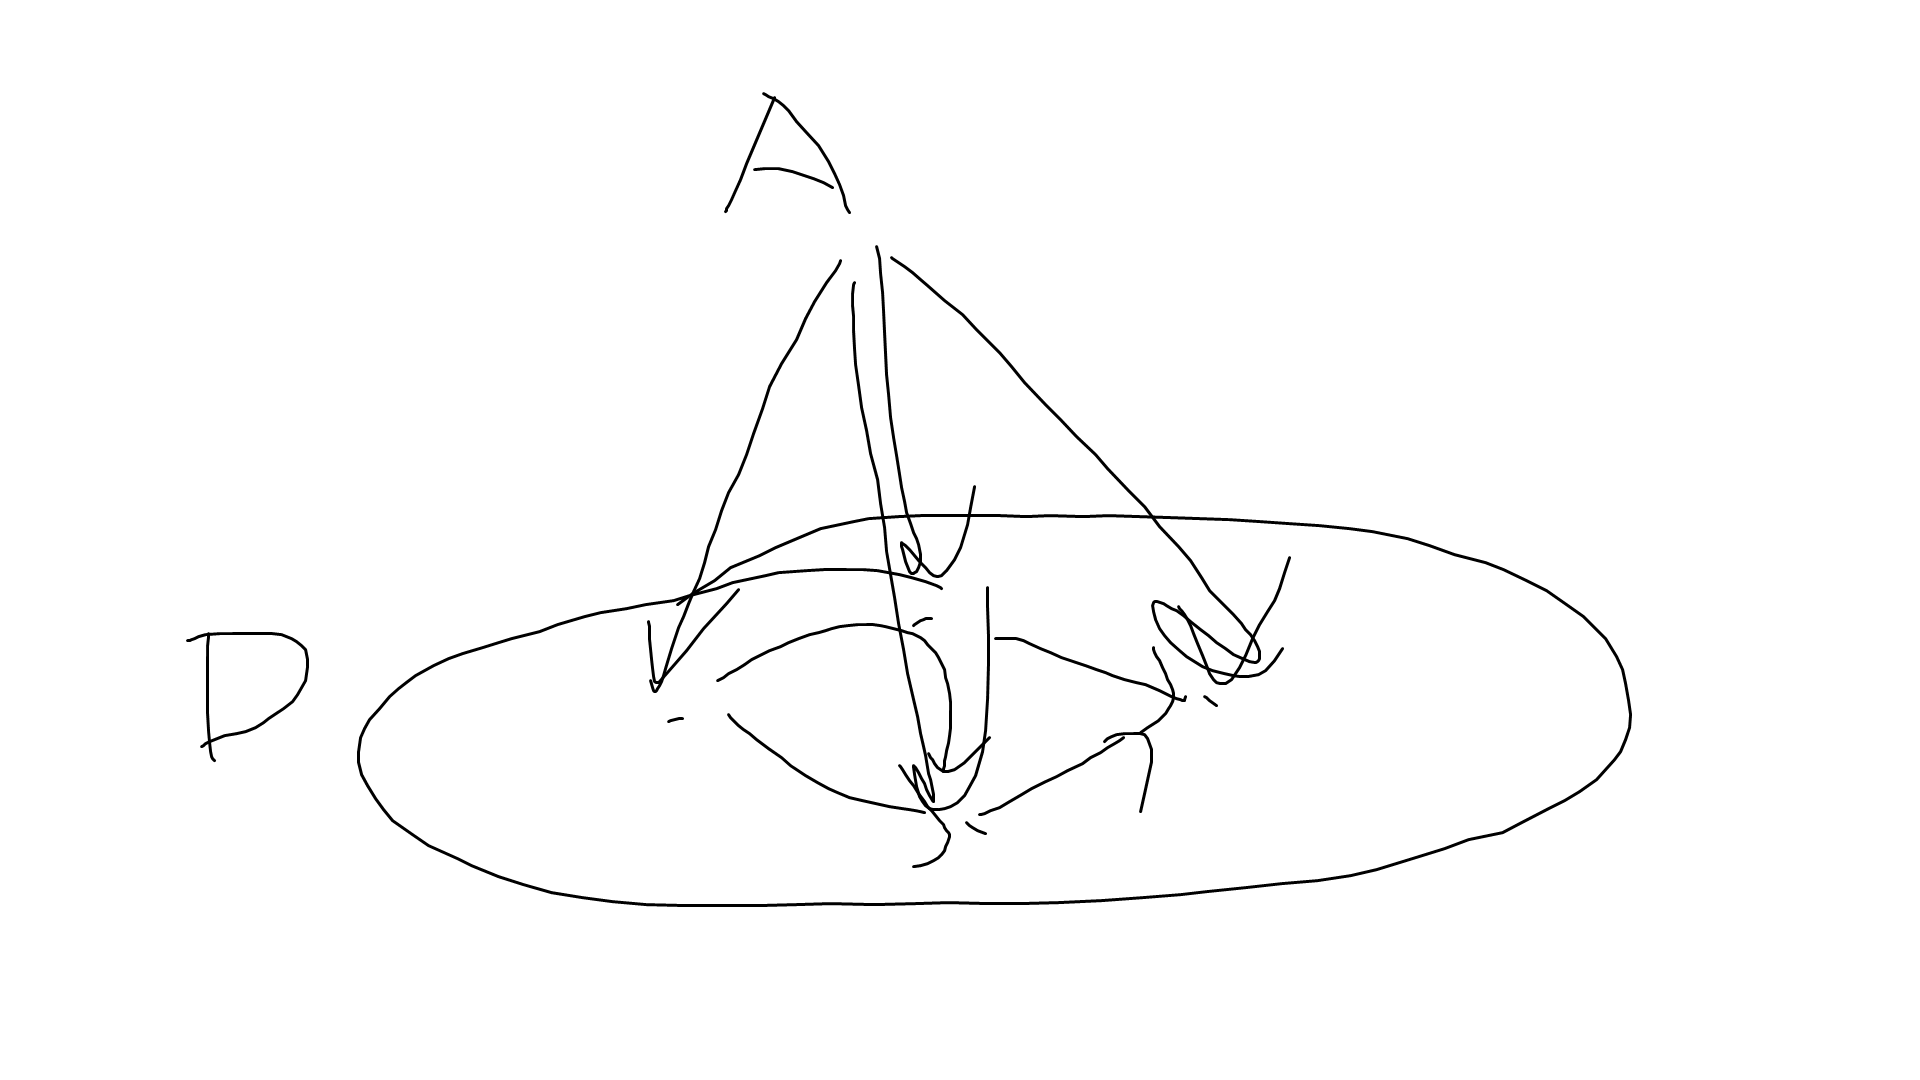
\includegraphics[scale=0.5]{image/Cat_07.png}

    Given cones $(A,(\lambda_j)_{j \in \ob \mathcal{J}})$ and $(B,(\mu_j)_{j \in \ob \mathcal{J}})$, a \emph{morphism} of cones between them is a morphism $A \xrightarrow{f} B$ s.t.
    \begin{tikzcd}
        A \arrow[rr,"f"] \arrow[rd,"\lambda_j"'] & & B \arrow[dl, "\mu_j"]\\
        & D(j) &
    \end{tikzcd}
    commutes for all $j$.

    We write $\mathbf{Cone}(D)$ for the category of cones over $D$ (I guess with morphisms being all the possible ones from above?).\\
    (c) A \emph{limit} for $D$ is a terminal object of $\mathbf{Cone}(D)$, if this exists.\\
    Dually, we have the notion of cone under a diagram, and of colimit ($=$ initial cone under $D$).\\
    Alternatively, if $\mathcal{C}$ is locally small, and $\mathcal{J}$ is small, we have a functor $\mathcal{C}^{op} \to \mathbf{Set}$ sending $A$ to the set of cones with apex $A$. A limit for $D$ is a representation of this functor.\\
    If $\triangle A$ denotes the constant diagram of shape $\mathcal{J}$ with all vetices $A$ and all edges $1_A$, then a cone over $D$ with apex $A$ is the same thing as a natural transformation $\triangle A \to D$.\\
    $\triangle$ is a functor $\mathcal{C} \to [\mathcal{J}, \mathcal{C}]$ and $\mathbf{Cone}(D)$ is the category $(\triangle \downarrow D)$ in the notation of ($3.3^{op}$) (the dual case of (3.3)...). So to say that every diagram of shape $J$ in $\mathcal{C}$ has a limit is equivalent to saying that $\triangle$ has a right adjoint. (We say $\mathcal{C}$ \emph{has limits} of shape $\mathcal{J}$).\\
    Dually, $\mathcal{C}$ has colimits of shape $J$ iff $\triangle:\mathcal{C} \to [\mathcal{J},\mathcal{C}]$ has a left adjoint.
\end{defi}

\begin{eg} (4.2)\\
    (a) (Lecturer says he'll give a very simple example) Suppose $\mathcal{J} = \phi$ (a diagram of that here. It's easy to draw, but a bit hard to see). There's a unique diagram of shape $\mathcal{J}$ in $\mathcal{C}$, a cone over it is just an object (with no legs), and a morphism of cones is a morphism of $\mathcal{C}$ (any one). So a limit for the empty diagram is a terminal object of $\mathcal{C}$.\\
    Dually, a colimit for it is an initial object.\\
    (Indeed a very simple example)

    ---Lecture 10---

    (b) Let $\mathcal{J}$ be the category with two objects and no non-identity morphisms. A diagram of shape $\mathcal{J}$ is a pair of objects $A,B$; a cone over it is a span
    \begin{tikzcd}
        & C \arrow[dl] \arrow[dr] &\\
        A & & B
    \end{tikzcd}
    ; and a limit for it is a product
    \begin{tikzcd}
        & A\times B \arrow[dl,"\pi_1"] \arrow[dr, "\pi_2"] &\\
        A & & B
    \end{tikzcd}
    as defined in 2.6(e). Dually, a colimit for it is a coproduct 
    \begin{tikzcd}
        A \arrow[dr,"\nu_1"] & & B \arrow[dl,"\nu_2"]\\
        & A+B &
    \end{tikzcd}

    (c) More generally, if $\mathcal{J}$ is a small discrete category, a diagram of shape $\mathcal{J}$ is a $\mathcal{J}$-indexed family $(A_j|j \in \mathcal{J})$, and a limit for it is a product $(\prod_{j \in J} A_j \xrightarrow{\pi_j} A_j | j \in \mathcal{J})$ (Dually, $(A_j \xrightarrow{\nu_j} \sum_{j \in \mathcal{J}} A_j | j \in \mathcal{J})$, or $\coprod_{j \in \mathcal{J}} A_j$, but we usually use the first notation).

    (d) Let $\mathcal{J}$ be the category 
    \begin{tikzcd}
        \cdot \arrow[r,shift left, "f"] \arrow[r, shift right, "g"'] & B
    \end{tikzcd}
    . A diagram of shape $\mathcal{J}$ is a parallel pair $A \stackrel[g]{f}{\rightrightarrows} B$; a cone over this is 
    \begin{tikzcd}
        & C \arrow[dl,"h"] \arrow[dr,"k"] &\\
        A & & B
    \end{tikzcd}
    satisfying $fh=k=gh$, or equivalently a morphism $C \xrightarrow{h} A$ satisfying $fh = gh$. A (co)limit for the diagram is a (co)equalizer as defined in 2.6(f).

    (e) Let $\mathcal{J}$ be the category
    \begin{tikzcd}
        & \cdot \arrow[d]\\
        \cdot \arrow[r] & \cdot
    \end{tikzcd}
    . A diagram of shape $\mathcal{J}$ is a cospan
    \begin{tikzcd}
        & A \arrow[d,"f"]\\
        B \arrow[r,"g"] & C
    \end{tikzcd} 
    , a cone over it is 
    \begin{tikzcd}
        D \arrow[r,"p"] \arrow[d,"q"] \arrow[dr, "r"] & A\\
        B & C
    \end{tikzcd}
    satisfying $fp=r=gq$, or equivalently, a span $(p,q)$ completing the diagram to a commutative square. A limit for the diagram is called a \emph{pullback} of $(f,g)$. In $\mathbf{Set}$, the apex of the pullback is the \emph{fibre product}
    $$ A \times_C B = \{(x,y) \in A \times B | f(x) = g(y)\}$$
    Dually, colimits of shape $\mathcal{J}^{op}$ are called \emph{pushouts}. Given 
    \begin{tikzcd}
        A \arrow[r,"f"] \arrow[d,"g"] & B\\
        C & \\
    \end{tikzcd}
    , we \emph{push $g$ along $f$} to get the RH side of the colimit square.

    (f) (not very important for this course, but might explain why the term \emph{limit} is used) Let $J$ be the poset of natural numbers. A diagram of shape $J$ is a \emph{direct system} $A_0 \xrightarrow{f_0} A_1 \xrightarrow{f_1} A_2 \xrightarrow{f_2} ...$\\
    A colimit for this is called a \emph{direct limit}: it consists of $A_\infty$ equipped with morphisms $A_n \xrightarrow{g_n} A_\infty$ satisfying $g_n = g_{n+1}$ for all $n$, and universal among such.\\
    Dually, we have \emph{inverse system} and \emph{inverse limit}.
\end{eg}

\begin{thm} (4.3)\\
    (i) Suppose $\mathcal{C}$ has equalizers and all finite (respectively, small) products. Then $\mathcal{C}$ has all finite (respectively, small) limits.\\
    (ii) Suppose $\mathcal{C}$ has pullbacks and a terminal object, then $\mathcal{C}$ has all finite limits.
    \begin{proof}
        (i) Suppose given $D:\mathcal{J} \to \mathcal{C}$. Form the products $P=\prod_{j \in \ob\mathcal{J}} D(j)$ and $Q = \prod_{\alpha \in \mor\mathcal{J}} D(\cod \alpha)$.\\
        We have morphisms $P \stackrel[g]{f}{\rightrightarrows} Q$ defined by $\pi_\alpha f = \pi_{\cod(\alpha)}$, $\pi_\alpha g = D(\alpha) \pi_{\dom \alpha}$ for all $\alpha$.\\
        Let $E \xrightarrow{e} P$ be an equalizer of $(f,g)$. The composites $\lambda_j = \pi_j e: E \to D(j)$ form a cone over $D$: given $\alpha: j \to j'$ in $\mathcal{J}$, 
        $$D(\alpha) \lambda_j = D(\alpha) \pi_j e = \pi_\alpha ge = \pi_\alpha fe = \pi_{j'} e = \lambda_{j'}$$
        Given any cone $(A,(\mu_j | j \in \ob\mathcal{J}))$ over $D$, there's a unique $\mu:A \to P$ with $\pi_j \mu = \mu_j$ for each $j$, and $\pi_\alpha f \mu = \mu_{\cod \alpha} = D(\alpha) \mu_{\dom \alpha} = \pi_\alpha g\mu$ for all $\alpha$, and hence $f\mu = g\mu$. So there is a unique $\nu:A \to E$ with $e\nu = \nu$. So $(E,(\lambda_j | j \in \ob \mathcal{J}))$ is a limit cone.

        (ii) It's enough to construct finite products and equalizers. But if $1$ is the terminal object, then a pullback for 
        \begin{tikzcd}
                        & A \arrow[d]\\
            B \arrow[r] & 1
        \end{tikzcd}
        has the universal property of a product $A \times B$, and we can form $\prod_{i=1}^n A_i$ inductively as $A_1 \times (A_2 \times (A_3 \times ... (A_{n-1} \times A_n)))$.\\
        Now, to form the equalizer of $A \stackrel[g]{f}{\rightrightarrows} B$, consider the cospan
        \begin{tikzcd}
            & A \arrow[d,"{(1_A,f)}"]\\
            A \arrow[r,"{(1_A,g)}"] & A \times B
        \end{tikzcd}
        . A cone over this consists of 
        \begin{tikzcd}
            P \arrow[r,"h"] \arrow[d,"k"] & A\\
            A &
        \end{tikzcd}
        satisfying $(1_A,f) h = (1_A,g) k$, or equivalently $1_A h = 1_A k$, and $fh = gk$, or equivalently, a morphism $P \xrightarrow{h} A$ satisfying $fh = gh$ (think). So a pullback for $(1_A,f)$ and $(1_A,g)$ is an equalizer of $(f,g)$.\\
        We say a category $\mathcal{C}$ is \emph{complete} if it has all small limits. Dually, \emph{cocomplete} means it has all small colimits.\\
        $\mathbf{Set}$ is both complete and cocomplete: products are cartesian products, coproducts are disjoint unions.\\
        Similarly, $\mathbf{Gp}$, $\mathbf{AbGp}$, $\mathbf{Rng}$, $\mathbf{Mod}_R$,... are all complete and cocomplete (nice to know that). $\mathbf{Top}$ is also complete and cocomplete, ...
    \end{proof}
\end{thm}

\begin{defi} (4.4)\\
    Let $F: \mathcal{C} \to \mathcal{D}$ be a functor.\\
    (a) We say $F$ \emph{preserves limits} of shape $\mathcal{J}$ if, given $D:\mathcal{J} \to \mathcal{C}$ and a limit cone $(L,(\lambda_j|j \in \ob\mathcal{J}))$ in $\mathcal{C}$, $(FL, (F\lambda_j | j \in \ob \mathcal{J}))$ is a limit for $FD$.\\
    (b) We say $F$ \emph{reflects limits} of shape $\mathcal{J}$ if, given $D:\mathcal{J} \to \mathcal{C}$ and a cone $(L,(\lambda_j)_j)$ s.t. $(FL,(F\lambda_j)_j)$ is a limit for $FD$, then $(L,(\lambda_j)_j)$ is a limit for $D$.\\
    (c) We say $F$ \emph{creates limits} of shape $\mathcal{J}$ if, given $D : \mathcal{J} \to \mathcal{C}$ and (lecturer had \emph{and and} here; if this is any other course I won'd bother put this, but this is Category Theory) a limit $(M,(\mu_j)_j)$ for $FD$, there exists a cone $(L,(\lambda_j)_j)$ over $D$ whose image under $F$ is isomorphic to the limit cone, and any such cone is a limit in $\mathcal{C}$. (This is stronger than both of above and implies them. Note that a lot of textbooks get this wrong; the definitions given by them are usually not categorical)
\end{defi}

---Lecture 11---

\begin{rem} (4.5)\\
    (a) If $\mathcal{C}$ has limits of shape $\mathcal{J}$, $F: \mathcal{C} \to \mathcal{D}$ preserves them and $F$ reflects isomorphisms, then $F$ reflects limits of shape $\mathcal{J}$ (???????).
    (b) $F$ reflects limits of shape $1$ $\iff$ $F$ reflects isomorphisms.\\
    (c) If $\mathcal{D}$ has limits of shape $\mathcal{J}$ and $F:\mathcal{C} \to \mathcal{D}$ creates them, then $F$ both preserves and reflects them.\\
    (d) In any of the statements of (4.3), we may replace both instances of \emph{$\mathcal{C}$ has} by either \emph{$\mathcal{C}$ has and $F:\mathcal{C} \to \mathcal{D}$ preserves} or \emph{$\mathcal{D}$ has and $F:\mathcal{C} \to \mathcal{D}$ creates}.
\end{rem}

We shall have some examples, as usual.

\begin{eg} (4.6)\\
    (a) $U : \mathbf{Gp} \to \mathbf{Set}$ creates all small limits: given a family $(G_i | i \in I)$ of groups, there's a unique group structure on $\prod_{i \in I} UG_i$ making the projections $\pi_i$ into homomorphisms, and this makes it into a product in $\mathbf{Gp}$.\\
    Similarly for equalizers (check).\\
    But $U$ doesn't preserve coproducts; $U(G * H) \not\cong UG \coprod UH$.\\
    (b) $U:\mathbf{Top} \to \mathbf{Set}$ preserves all small limits and colimits, but this times it doesn't reflect them: if $L$ is a limit for $D: \mathcal{J} \to \mathbf{Top}$, and $L$ is not discrete, there's another cone with apex $L_d$ (take the underlying set and \emph{retopologize} with discrete topology) mapping to the limit in $\mathbf{Set}$.\\
    (c) The inclusion functor $I:\mathbf{AbGp} \to \mathbf{Gp}$ reflects coproducts, but doesn't preserve them: the direct sum $A \oplus B$ (coproducts in $\mathbf{AbGp}$) is not normally isomorphic to the free product $A*B$; $A*B$ is not abelian unless either $A$ or $B$ is $\{e\}$.\\
    But if $A \cong \{e\}$, then $A*B \cong A \oplus B \cong B$.
\end{eg}

\begin{lemma} (4.7)\\
    If $\mathcal{D}$ has limits of shape $\mathcal{J}$, then so does the functor category $[\mathcal{C},\mathcal{D}]$ for any $\mathcal{C}$, and the forgetful functor $[\mathcal{C},\mathcal{D}] \to \mathcal{D}^{\ob \mathcal{C}}$ creates them.
    \begin{proof}
        Suppose given a diagram of shape $\mathcal{J}$ in $[\mathcal{C},\mathcal{D}]$; think of it as a functor $D:\mathcal{J} \times \mathcal{C} \to \mathcal{D}$. For each $A \in \ob\mathcal{C}$, let $(LA,(\lambda_{j,A}|j \in \ob \mathcal{J}))$ be a limit cone for the diagram $D(-,A): \mathcal{J} \to \mathcal{D}$.\\
        Given $A \xrightarrow{f} B$ in $\mathcal{C}$, the composites $LA \xrightarrow{\lambda_{j,A}} D(j,A) \xrightarrow{D(j,f)} D(j,B)$ form a cone over $D(-,B)$, since the sqaures 
        \begin{tikzcd}
            D(j,A) \arrow[r,"{D(j,f)}"] \arrow[d,"{D(\alpha,A)}"] & D(j,B) \arrow[d,"{D(\alpha,B)}"]\\
            D(j',A) \arrow[r,"{D(j',f)}"] & D(j',B)
        \end{tikzcd}
        commute. So there's a unique $LF:LA \to LB$ making
        \begin{tikzcd}
            LA \arrow[r,"{\lambda_{j,A}}"] \arrow[d,"Lf"] & D(j,A) \arrow[d,"{D(j,f)}"]\\
            LB \arrow[r,"{\lambda_{j,B}}"] & D(j,B)
        \end{tikzcd}
        commute for all $j$.\\
        As usual, uniqueness implies functoriality: given $g:B \to C$, $L(gf)$ and $(Lg)(Lf)$ are factorizations of the same cone through the limit $LC$. And this is the unique functor structure on $(A \to LA)$ making the $\lambda_{j,-}$ into natural transformations.\\
        The cone $(L,(\lambda_{j,-} | j \in \ob\mathcal{J}))$ is a limit: suppose given another cone $(M,(\mu_{j,-} | j \in \ob\mathcal{J}))$, then for each $A$, $(MA,(\mu_{j,A} | j \in \ob\mathcal{J}))$ is a cone over $D(-,A)$, so induces a unique $\alpha_A:MA \to LA$. Naturality of $\alpha$ follows from uniqueness of factorizations through a limit. So $(M,(\mu_j))$ factors uniquely through $(L,(\lambda_j))$.
    \end{proof}
\end{lemma}

\begin{rem} (4.8)\\
    Now we can prove something that I promised very long ago (see Sheet 1 Q4 as well). In any category, a morphism $A \xrightarrow{f} B$ is monic iff
    \begin{tikzcd}
        A \arrow[r,"1_A"] \arrow[d,"1_A"] & A \arrow[d,"f"]\\
        A \arrow[r,"f"] & B
    \end{tikzcd}
    is a pullback. Hence any functor which preserves pullbacks preserves monomorphisms.\\
    In particular, if $\mathcal{D}$ has pullbacks, then monomorphisms in $[\mathcal{C},\mathcal{D}]$ are just pointwise monomorphisms.\\
    The dual is the statement in comment of Sheet 1 Q4.
\end{rem}

\begin{thm} (4.9)\\
    Suppose $G:\mathcal{D} \to \mathcal{C}$ has a left adjoint $F$. Then $G$ preserves all limits which exist in $\mathcal{D}$.\\
    We'll present two proofs: the first (slick) proof is more for you to understand why this is true, while the second proof is more elementary.
    \begin{proof} (1)\\
        Suppose $\mathcal{C}$ and $\mathcal{D}$ both have limits of shape $\mathcal{J}$. We have a commutative diagram
        \begin{tikzcd}
            \mathcal{C} \arrow[r,"F"] \arrow[d,"\triangle"] & \mathcal{D} \arrow[d,"\triangle"]\\
            \left[\mathcal{J},\mathcal{C}\right] \arrow[r,"{[\mathcal{J},F]}"] & \left[\mathcal{J},\mathcal{D}\right]
        \end{tikzcd}
        , and all functors in it have right adjoints.\\
        In particular, $([\mathcal{J},F] \dashv [\mathcal{J},G])$.\\
        So by (3.6), the diagram of right adjoints
        \begin{tikzcd}
            \mathcal{D} \arrow[r,"G"] & \mathcal{C}\\
            \left[\mathcal{J},D\right] \arrow[u,"\lim_{\mathcal{J}}"] \arrow[r,"{[\mathcal{J},G]}"] & \left[\mathcal{J},\mathcal{C}\right] \arrow[u,"\lim_{\mathcal{J}}"]
        \end{tikzcd}
        commutes up to isomorphism, i.e. $G$ preserves limits of shape $\mathcal{J}$.\\
        This is the real reason why this theorem works, because right adjoint commute with right adjoints.\\
        However, this proof won't work if we don't know we have limits.
    \end{proof}

    \begin{proof} (2)\\
        Suppose given $D:\mathcal{J} \to \mathcal{D}$ and a limit cone $(L,(L \xrightarrow{\lambda_j} D(j) | j \in \ob \mathcal{J}))$. Given a cone $(A,(A \xrightarrow{\alpha_j} GD(j) | j \in \ob\mathcal{J}))$ over $GD$, the morphisms $FA \xrightarrow{\hat{\alpha}_j} D(j)$ form a cone over $D$, so they induce a unique $FA \xrightarrow{\hat{\beta}} L$ such that $\lambda_j \hat{\beta} = \hat{\alpha}_j$ for all $j$.\\
        Then $A \xrightarrow{\beta} GL$ is the unique morphism satisfying $(G \lambda_j) \beta = \alpha_j$ for all $j \in \mathcal{J}$. So $(GL,(G\lambda_j | j \in \ob\mathcal{J}))$ is a limit cone in $\mathcal{C}$.\\
        The \emph{primeval Adjoint Functor Theorem} says that the converse of (4.9) is true: if $\mathcal{D}$ has (limits), and $G:\mathcal{D} \to \mathcal{C}$ preserves \emph{all} limits, then $G$ has a left adjoint.
    \end{proof}
\end{thm}

---Lecture 12---

Second example class: Friday 9 November, 14:00, MR3.

\begin{lemma} (4.10)\\
    Suppose $\mathcal{D}$ has and $G:\mathcal{D} \to \mathcal{C}$ preserves limits of shape $\mathcal{J}$. Then for any $A \in \ob \mathcal{C}$, the arrow category $(A \downarrow G)$ has limits of shape $\mathcal{J}$, and the forgetful functor $U:(A \downarrow G) \to \mathcal{D}$ creates them.
    \begin{proof}
        Suppose given $D:\mathcal{J} \to (A\downarrow G)$; write $D(j)$ as $(UD(j),f_j)$.\\
        Let $(L,(\lambda_j:L \to UD(j))_{j \in \ob\mathcal{J}}$ be a limit for $UD$; then $(GL,(G\lambda_j)_{j \in \ob\mathcal{J}})$ is a limit for $GUD$. Since the edges of $UD$ are morphisms in $(A \downarrow G)$, the $f_j$ form a cone over $GUD$.\\
        So there's a unique $h:A \to GL$ s.t. $(G\lambda_j)h = f_j$ for all $j$, i.e. there is a unique $h$ s.t. the $\lambda_j$ are all morphisms $(L,h) \to (UD(j),f_j)$ in $(A \downarrow G)$.\\
        We need to show that $((L,h),(\lambda_j)_{j \in \ob\mathcal{J}})$ is a limit cone in $(A \downarrow G)$.\\
        If $((C,k),(\mu_j)_{j \in \ob\mathcal{J}})$ is any cone over $D$, then $(C,(\mu_j)_{j \in \ob\mathcal{J}})$ is a cone over $UD$. So there's a unnique $l:C \to L$ with $\lambda_j l = \mu_j$ for all $j$. We need to show $(Gl)k = h$: but $(G\lambda_j) (Gl)k = (G\mu_j)k = f_j = (G\lambda_j) h$ for all $j$. So $(Gl)k = h$ by uniqueness of factorizations through limits.
    \end{proof}
\end{lemma}

\begin{lemma} (4.11)\\
    A category $\mathcal{C}$ has an initial object iff $1_{\mathcal{C}}:\mathcal{C} \to \mathcal{C}$, regarded as a diagram of shape $\mathcal{C}$ in $\mathcal{C}$, has a limit.
    \begin{proof}
        First, suppose $\mathcal{C}$ has an initial object $I$. Then the unique morphisms $(I \to A | A \in \ob\mathcal{C})$ form a cone over $1_{\mathcal{C}}$; and given any cone $(C \xrightarrow{\lambda_A} A |A \in \ob\mathcal{C})$, then for any $A$ the triangle 
        \begin{tikzcd}
            C \arrow[rd,"\lambda_A"] \arrow[r,"\lambda_I"] & I \arrow[d]\\
            & A
        \end{tikzcd}
        commutes, so $\lambda_I$ is the unique factorization of $(\lambda_A|A \in \ob\mathcal{C})$ through $(I \to A|A\in\ob\mathcal{C})$.\\
        Conversely, suppose $(I,(\lambda_A:I \to A|A \in \ob\mathcal{C}))$ has a limit. Then for any $I \xrightarrow{f} A$, the diagram
        \begin{tikzcd}
            I \arrow[r,"\lambda_I"] \arrow[rd,"\lambda_A"] & I \arrow[d,"f"]\\
            & A
        \end{tikzcd}
        commutes. In particular, putting $f = \lambda_A$, we see that $\lambda_I$ is a factorization of the limit cone through itself, so $\lambda_I = 1_I$. Hence every $f:I \to A$ satisfies $f=\lambda_A$. So $I$ is initial.
    \end{proof}
\end{lemma}

The primeval adjoint functor theorem follows immediately from (4.10), (4.11) and (3.3).\\
However, it only applies to functors between preorders (since that's the only category that satisfies the conditions; c.f. Sheet 2 Q6).

\begin{thm} (4.12, General Adjoint Functor Theorem)\\
    Suppose that $\mathcal{D}$ is locally small and complete. Then $G:\mathcal{D} \to \mathcal{C}$ has a left adjoint $\iff$ $G$ preserves all small limits (some people use the word \emph{continuous} for this) and, for each $A \in \ob\mathcal{C}$, there exists a \emph{set} of morphisms $\{A \xrightarrow{f_i} GB_i | i \in I\}$ s.t. every $A \xrightarrow{h} GC$ factors as $A \xrightarrow{f_i} GB_i \xrightarrow{Gg} GC$ for some $i$ and some $g:B_i \to C$.\\
    (We say $G$ satisfies the \emph{solution set condition}.)
    \begin{proof}
        $\implies$: If $(F \dashv G)$, $G$ preserves limits by (4.9), and $\{A \xrightarrow{\eta_A} GFA\}$ is a singleton solution set, by (3.3).\\
        $\Leftarrow$: By (4.10) $(A\downarrow G)$ is complete, and it inherits local smallness from $\mathcal{D}$. So we need to show: if $\mathcal{A}$ is compelte and locally small, and has a weakly initial set of objects $\{B_i | i \in I\}$, then $\mathcal{A}$ has an initial object.\\
        First form $P=\prod_{i \in I} B_i$, then $P$ is weakly initial. Now form the limit of $P \stackrel[\to]{\to}{...} P$ (*) whose edges are all the endomorphisms of $P$; denote it $I \xrightarrow{i} P$. $I$ is also weakly initial in $\mathcal{A}$; suppose given $I \stackrel[g]{f}{\rightrightarrows} C$. Form equalizer $E \xrightarrow{e} I$ of $(f,g)$; then there exists $P\xrightarrow{h} E$ since $P$ is weakly initial.\\
        $ieh:P \to P$ and $1_P$ are edges of the diagram (*) above, so $i=iehi$. But $i$ is monic, so $ehi = 1_I$; in particular, $e$ is split epic. So $f=g$.\\
        Hence $I$ is initial.
    \end{proof}
\end{thm}

\begin{eg} (4.13)\\
    (a) Suppose you've never heard of free groups nor how to construct them. Consider the forgetful functor $U: \mathbf{Gp} \to \mathbf{Set}$. By (4.6 a), $U$ creates all small limits, so $\mathbf{Gp}$ has them and $U$ preserves them. $\mathbf{Gp}$ is locally small; now given a set $A$, any $f:A \to UG$ factors as $A \to UG' \to UG$, where $G' \leq G$ is the subgroup generated by $\{f(x) |x \in A\}$, and $\Card G' \leq \max\{\aleph_0,\Card A\}$.\\
    Let $B$ be a set of this cardinality, and consider all possible subsets $B' \subseteq B$. All group structures on $B'$ and all mappings $A \to B'$. So these give us a solution set at $A$.\footnote{However this is not a very good example -- how did we know the upper bound of $\Card G'$? We knew it because we've already known free group consists of all words generated by set elements. Indeed this is almost always the case: if you've known enough about the functor so that you can find a solution set to apply GAFT, almost always you could have constructed the adjoint explicitly.}\\
    (b) Consider the category $\mathbf{CLat}$ of complete lattices, i.e. posets with all meets and joins. Again, $U:\mathbf{CLat} \to \mathbf{Set}$ creates all small limits. But A.W.Hales (1964) showed that, for any cardinal $\kappa$, there exist complete lattices of cardinality $\geq \kappa$ generated by three elements; so the SSC fails at $A=\{x,y,z\}$. Hence $U$ doesn't have a left adjoint.
\end{eg}

---Lecture 13---

\begin{defi} (4.14)\\
    By a \emph{subobject} of an object $A$ of $\mathcal{C}$, we mean a monomorphism $A' \rightarrowtail A$. The subobjects of $A$ are preordered by $A'' \leq A'$, if there exists a factorization 
    \begin{tikzcd}
        A'' \arrow[rr] \arrow[rd,tail] & & A' \arrow[ld, tail]\\
        & A &
    \end{tikzcd}
    i.e. a factorization of $A''$ through $A'$.\\
    We say $\mathcal{C}$ is \emph{well-ordered} if each $A \in \ob\mathcal{C}$ has a set of subobjects $\{A_i \rightarrowtail A | i \in I\}$ s.t. every subobject of $A$ is isomorphic to some $A_i$ (e.g. in $\mathbf{Set}$ we can take the inclusions $\{A' \hookrightarrow A| A'\in PA\})$.\\
    If $\mathcal{C}^{op}$ is well-powered, we say $\mathcal{C}$ is \emph{well-copowered}\footnote{Some people use \emph{cowell-powered}, but lecturer thought that meant \emph{not well-powered} so decided not to use that.}. 
\end{defi}

\begin{lemma} (4.15)\\
    Suppose given a pullback square
    \begin{tikzcd}
        P \arrow[r,"h"] \arrow[d,"k"] & A \arrow[d,tail,"f"]\\
        B \arrow[r,"g"] & C
    \end{tikzcd}
    with $f$ monic. Then $k$ is monic.
    \begin{proof}
        Suppose $D \stackrel[y]{x}{\rightrightarrows} P$ satisfy $kx=ky$. Then $fhx=gkx=gky=fhy$. But $f$ is monic, so $hx=hy$. So $x$ and $y$ are factorizations of the same cone through the limit cone $(h,k)$.
    \end{proof}
\end{lemma}

\begin{thm} (4.16, Special AFT)\\
    Suppose $\mathcal{C}$ and $\mathcal{D}$ are both locally small, and that $\mathcal{D}$ is complete and well-powered and has a coseparating set (see (2.8)). Then a functor $G:\mathcal{D} \to \mathcal{C}$ has a left adjoint iff it preserves all small limits.
    \begin{proof}
        $\implies$: by (4.9).\\
        $\Leftarrow$: For any $A \in \ob\mathcal{C}$, $(A \downarrow G)$ is complete by (4.10), locally small, and well-powered, since the subobjects of $(B,f)$ in $(A\downarrow G)$ are just those subobjects $B' \rightarrowtail B$ in $\mathcal{D}$ for which $f$ factors through $GB' \rightarrowtail GB$.\\
        Also, if $\{S_i | i \in I\}$ is a coseparating set for $\mathcal{D}$, then the set $\{(S_i, f)|i \in Im f \in \mathcal{C}(A,GS_i)\}$ is coseparating in $(A \downarrow G)$: given $(B,f) \stackrel[h]{g}{\rightrightarrows} (B',f')$ in $(A \downarrow G)$ with $g \neq h$, there exists some morphism $k:B' \to S_i$ for some $i$ with $kg \neq kh$, and then $k$ is also a morphism $(B',f') \to (S_i,(Gk)f')$ in $(A \downarrow G)$.\\
        So we need to show that if $\mathcal{A}$ is complete, locally small and well-powered and has a coseparating set $\{S_i|i \in I\}$, then $\mathcal{A}$ has an initial object: form the product $P=\prod_{i \in I} S_i$. Now consider the diagram

        \begin{tikzcd}
            & & & & P_i \arrow[ddd, tail]\\
            & & P_j \arrow[ddrr, tail] \arrow[lldd, bend right = 15, dotted, no head] & &\\
            & & & &\\
            P' \arrow[rrrr,tail] & & & & P
        \end{tikzcd}

        whose edges are a representative set of subobjects of $P$, and form its limit

        \begin{tikzcd}
            I \arrow[rrr] \arrow[rrd] \arrow[ddd] & & & P_i\\
            & & P_j \arrow[lldd, dotted, no head, bend left = 15] &\\
            & & &\\
            P' & & &
        \end{tikzcd}

        By the argument of (4.15), the legs of this cone are all monic; in particular, $I \rightarrowtail P$ is monic, and it's a least subobject of $P$. Hence $I$ has no proper subobjects.\\
        So, given $I \stackrel[g]{f}{\rightrightarrows} A$, their equalizer is an isomorphism, hence $f=g$.\\
        Now let $A$ be any object of $\mathcal{A}$; form the product
        $$Q = \prod_{i \in I, f \in \mathcal{A}(A,S_i)} S_i$$
        There's an \emph{obvious} $h:A \to Q$ defined by $\pi_{i,f} h = f$; and $h$ is monic, since the $S_i$ are a coseparating set.\\
        We alsk have a morphism $k:P \to Q$ defined by $\pi_{i,f} k = \pi_i$.\\
        Now form the pullback 
        \begin{tikzcd}
            B \arrow[r] \arrow[d,tail] & A \arrow[d,tail,"h"]\\
            P \arrow[r,"k"] & Q
        \end{tikzcd}
        ; by (4.15), $P$ is monic, so $B$ is a subobject of $P$. Hence there exists 
        \begin{tikzcd}
            I \arrow[rr] \arrow[rd] & & B \arrow[ld]\\
            & P &
        \end{tikzcd}
        hence a morphism $I \to B \to A$.\footnote{This proof was first mentioned in a book where the author left as an exercise to the readers}
    \end{proof}
\end{thm}

\begin{eg} (4.17)\\
    Consider the inclusion $\mathbf{KHaus} \xrightarrow{I} \mathbf{Top}$, where $\mathbf{KHaus}$ is the full subcategory of compact Hausdorff spaces (see (3.11 b)). $\mathbf{KHaus}$ has, and $I$ preserves all small products (by Tychonoff's theorem), and equalizers (since equalizers of pairs $X\stackrel[g]{f}{\rightrightarrows} Y$ with $Y$ Hausdorff are closed subspaces).\\
    Both categories are locally small and $\mathbf{KHaus}$ is well-powered (subobjects of $X$ are all isomorphic to closed subspaces). The closed intervals $[0,1]$ is a coseparator in $\mathbf{KHaus}$, by Uryson's Lemma which is well-known in Topology (ok). So we have everything in (4.16), so this functor $I$ has a left adjoint $\beta$ (known as \href{https://en.wikipedia.org/wiki/Stone%E2%80%93%C4%8Cech_compactification}{\emph{Stone-\u{C}ech compactification}}).
\end{eg}

\begin{rem} (4.18)\\
    (a) We've proved the existence in above, but it might also be interesting to see how $\beta$ actually might look like.\\
    \u{C}ech's construction of $\beta$: given $X$, form $Q = \prod_{f:X \to [0,1]} [0,1]$ and define $h:X \to P$ by $\pi_f h = f$. Define $\beta X$ to be the closure of the image of $h$.\\
    \u{C}ech's proof that this works is essentially the same as (4.16).\\
    (b) We could have used GAFT to construct $\beta$ as well: we get a solution set at $X$ by considering all continuous $X \xrightarrow{f} Y$ with $Y$ compact Hausdorff, and $\im f$ dense in $Y$ and such $Y$ have cardinality at most $2^{2^{\Card X}}$.
\end{rem}










\newpage

\section{Example Class 1}
Many people wrote too much for questions. Do have the confidence to use the duality principle when it's usable!

\subsection{Question 1}
We do need to verify
\begin{equation*}
    \begin{aligned}
        ((AB)C)_{il} &= \vee_k ((\vee_j (a_{ij} \wedge b_{jk} )) \wedge c_{kl})\\
        &= \vee_k \vee_j (a_{ij} \wedge b_{jk} \wedge c_{kl})\\
        &= (A(BC))_{il} \text{ by symmetry}
    \end{aligned}
\end{equation*}
and of course identity matrices are identities.

Define a functor $F:\mathbf{Mat}_L \to \mathbf{Rel}_f$ by $F(n) = \{1,2,...,n\}$; if $A: n \to p$ is a $p \times n$ matrix in $\mathbf{Mat}_L$, then $FA = \{(i,j) | a_{ji} = 1\}$.\\
Important: we have to verify this is functorial, which many people didn't bother to do. Why is it functorial? Well again we just have to verify explicitly that
\begin{equation*}
    \begin{aligned}
        (AB)_{ik} = 1 \iff (\exists j) (a_{ij} = b_{jk} = 1)
    \end{aligned}
\end{equation*}
so $F(AB) = FA \circ FB$. This does require verifications, because you are multiplying the matrices over lattices; for example say if you are doing it for the finite field with 2 elements then it won't work.\\
Now note that to prove they are equivalent we don't really need to find both the two functors and natural transformations; instead we can use a theorem in chapter 1, that $F$ is part of an equivalence if it is full, faithful and essentially surjective. So we just have to verify that $F$ is f,f,and es. Indeed it is, since any finite set is isomorphic to $F(n)$ for some $n$. So by (1.12), $\mathbf{Mat}_L \simeq \mathbf{Rel}_f$.

\subsection{Question 2}
Part (i) was easy, but many people had problems on part (ii).\\
(i) Given $(A_i | i \in I)$, define $\mathcal{C}$ by $\ob \mathcal{C} =\{(i,a)| i \in I, a \in A_i\}$, and $\mathcal{C}((i,a)(j,b)) = \phi$ if $i \neq j$, and is $\{*\}$ if $i=j$.\\
$\mathcal{C}$ is a groupoid; its isomorphic classes of objects are of the form $\{i\} \times A,i \in I$. If we've got a skeleton then we can pick out one from each of these, which is equivalent to AC.\\
(ii) Now take $\ob\mathcal{C} =I\times \{0,1\}$, and morphisms $(i,m) \to (i,n)$ are formal finite sums as given in the hint, and of course composition is just addition. Again this is a groupoid because every morphism can be inverted by just reverting the sign of every coefficient. So $\mathcal{C}$ has isomorphic classes $\{i\} \times \{0,1\}, i \in I$. So this has a skeleton, say we take $\mathcal{C}_0$ to be the full subcategory on objects $I\times\{0\}$.\\
But then by assumption we have an equivalence $\mathcal{C}_0 \stackrel[G]{F}{\rightleftarrows} \mathcal{C}$, then $FG(i,0) = FG(i,1)$ for all $i$. So if we have a natural transfomation $\beta:FG \to 1_{\mathcal{C}}$ which is also an isomorphism, then either $\beta_{(i,0)}$ or $\beta_{(i,1)}$ is a non-zero formal finite sum. So we just put $A_i = \{x \in A_i | x$ occurs in either $\beta_{(i,0)}$ or $\beta_{(i,1)}$ with non-zero coefficient$\}$.

\subsection{Question 3}
(i) Quite a lot of people forgot to verify that it is actually a subgroup! Suppose given automorphisms $F,G,H$ with isomorphisms $\alpha:F \to 1_{\mathcal{C}},\beta:G \to 1_{\mathcal{C}}$. Then $(F^{-1} \alpha)^{-1} : F^{-1} \to F^{-1}F = 1_{\mathcal{C}}$ is an isomorphism, so $F^{-1}$ is inner. Now $FG\xrightarrow{F\beta} F \xrightarrow{\alpha} 1_\mathcal{C}$ is isomorphism, so $FG$ is inner.\\
Now we have to verify normality: $HFH^{-1} \xrightarrow{H \alpha_{H^{-1}}} HH^{-1} = 1_{\mathcal{C}}$ is iso, so $HFH^{-1}$ is inner.\\
You don't have to spend a lot of time to verify that all these are nat transforms (ok).\\
(ii) Note that an isomorphism is in particular an equivalence. Now if $F$ is an automorphism, it is full and faithful, so for any $A$, morphism $A \to F1$ are in bijection with morphisms $F^{-1} A \to 1$, so there's just one of them.\\
Hence if $F$ is an isomorphism of $\mathbf{Set}$, $F(1) = 1$, and hence there's a unique $\alpha: \mathbf{Set} (1,-) \to F$ (this is just Yoneda).\\
We need to show $\alpha$ is iso: but for any $A$, and any $1 \xrightarrow{x} A$, 
\begin{tikzcd}
    1 \arrow[r,"\alpha_1"] \arrow[d,"x"] & F1 \arrow[d,"Fx"]\\
    A \arrow[r,"\alpha_A"] & FA
\end{tikzcd}
commutes, but $F$ is full and faithful, so $\alpha_A$ is bijective. Hence by (1.8), $\alpha$ is an isomorphism.\\
(iii) Note that if $X$ has $\geq 3$ points, then it has $\geq 4$ continuous endo maps (constants and identity). If $X$ has $\leq 1$ point, then its only endo is $1_X$. So the only possibility is $X$ having 2 points. Say $X = \{0,1\}$ wit discrete or indiscrete topology, all 4 maps $X \to X$ are continuous. So the only possible topology is the Sierpinski space given in the question (or the other way), which there are 3 continuous maps $X \to X$.\\
Hence if $F$ is an autom of $\mathcal{C} \subseteq \mathbf{Top}$, we must have $FS \cong S$.\\
We also have $F1 \cong 1$, and $U:\mathcal{C} \to \mathbf{Set}$ is iso to $\mathcal{C} (1,-)$. So there's a unique nat $\alpha: U \to UF$, and $\alpha_X$ is bijective for all $X$, as before. Now we don't know if $\alpha_X$ is continuous or not for a given $X$. So we consider naturality squares
\begin{tikzcd}
    UX \arrow[r,"\alpha_X"] \arrow[d,"Uf"] & UFX \arrow[d,"UFf"]\\
    US \arrow[r,"\alpha_S"] & UFS
\end{tikzcd}
. If $\alpha_S$ is discontinuous, then for any $X$, $\alpha_X$ maps open subsets of $X$ bijecively to closed subsets of $FX$, but this is impossible if not every intersection of open sets in $X$ is open.\\
So then $\alpha_S$ is a homeomorphism, and $\alpha_X$ is a homeomorphism for all $X$.\\
(iv) This basically says that if we restrict to finite topological spaces, then we do have the other case in the above happening. Let $F:\mathbf{Top}_f \to\mathbf{Top}_f$ sending $X$ to the same set with closed sets as new opens.\\
Then $FF = 1_{\mathbf{Top}_f}$, so $F$ is an automorphism, and it is not isomorphic to the identity as there exists finite spaces $X$ with $X \not\cong FX$ (we could find one with 3 points -- lecturer didn't give the explicit example). So $F$ is not inner.\\
Now if $G$ is any non-inner autom, then $GF$ is inner(?????); so $|\Aut(\mathbf{Top}_f):Inn(Top_f)| = 2$.

\subsection{Question 4}
(i) Suppose we are given 
\begin{tikzcd}
    C \arrow[r,"h"] \arrow[d,"g", two heads] & A \arrow[d,tail,"f"]\\
    D \arrow[r,"k"] & B \arrow[d,"p"',shift right] \arrow[d,"q", shift left]\\
    & E
\end{tikzcd}
where $f$ is an equalizer of $(p,q)$.\\
Then $pfh = pkg = qkg = qfh$, and $g$ is epic, so $pk = qk$, so exists unique $t$ with $ft=k$. Then $ftg = kg = fh$, and $f$ is monic, so $tg = h$.\\
(ii) 
\begin{tikzcd}
    A \arrow[dr,"k"] \arrow[r,"f"] & B \arrow[d,"g"',shift right] \arrow[d,"h", shift left] & D \arrow[l,"l"] \arrow[dl,"m"]\\
    & C &
\end{tikzcd}
Note that $f$ isn't regular monic. Why not? Because it is not iso and not an equalizer of $(g,h)$, since $l$ doesn't factor through it. It is trivially monic and strong monic: the only squares with $f$ on RHS is to put the identity before $f$, but it's trivial to verify those cases.\\
In some sense we can see that this is a minimal counter-example to the statement (think a bit, there's not anything better you can do).\\
(iii) This actually has nothing to do with the previous two parts. We have 
\begin{tikzcd}
    A \arrow[r,"f"] \arrow[rd,"k"] & B \arrow[d,"g"',shift right] \arrow[d,"h",shift left]\\
    & C
\end{tikzcd}
We want a commutative square
\begin{tikzcd}
    \cdot \arrow[r] \arrow[d] & \cdot \arrow[d]\\
    \cdot \arrow[r] & \cdot
\end{tikzcd}
with one vertical edge $f$ and the other one not. There are still a lot of possibilities, but almost any of it work. Say we pick
\begin{tikzcd}
    \cdot \arrow[r,"f"] \arrow[d,"f"] & \cdot \arrow[d,"g"]\\
    \cdot \arrow[r,"h"] & \cdot
\end{tikzcd}
Try $f,f,g,h$: the only possible composites are with 
\begin{tikzcd}
    \cdot \arrow[r,"h"] \arrow[d,"1_B"] & \cdot \arrow[d,"1_C"]\\
    \cdot \arrow[r,"h"] & \cdot
\end{tikzcd}
or 
\begin{tikzcd}
    \cdot \arrow[r,"h"] \arrow[d,"h"] & \cdot \arrow[d,"1_C"]\\
    \cdot \arrow[r,"1_C"] & \cdot
\end{tikzcd}
So $(f,g)$ is vacuously epic.

\subsection{Question 5}
This question has a lots of boring parts so lecturer is not going to write out all of it. The only a little bit tricky part is the strong part of (ii). We'll do that: suppose $gf$ is strong monic, and suppose we are given
\begin{tikzcd}
    \cdot \arrow[r,"l"] \arrow[d,"h", two heads] & \cdot \arrow[d,"f"]\\
    \cdot \arrow[r,"k"] & \cdot \arrow[d,"g"]\\
    & \cdot
\end{tikzcd}
. Then
\begin{tikzcd}
    \cdot \arrow[r,"l"] \arrow[d, "k", two heads] & \cdot \arrow[d,"gf", tail]\\
    \cdot \arrow[ru,"t", dashed] \arrow[r,"gk"] & \cdot
\end{tikzcd}
commutes. A lot of people used $g$ is monic, but we weren't given it here(oops)! Here $\exists t$ with $th = l$ (and $gft = gk$). Then $fth = fl = kh$ and $h$ is epic, so $ft = k$.\\
Suppose $gf$ is regular monic, say it's the equalizer of $\cdot \stackrel[l]{k}{\rightrightarrows} \cdot$. To show that $f$ is an equalizer of $(kg,fg)$, suppose we are given 
\begin{tikzcd}
    \cdot \arrow[r,"m"] & \cdot
\end{tikzcd}
with $kgm = lgm$. Then $\exists ! n$ with $gm = gfn$. But now $g$ is monic. So $m = fn$.\\
(iv) This part is also fairly problematic. The first thing we need to work out is what equalizers look like in this category. Given $A \stackrel[g]{f}{\rightrightarrows} B$ in $\mathcal{C}$, their equalizer in $\mathbf{AbGp}$ is the subgroup of $\{a \in A | f(a) = g(a)\}$, and this belongs to $\mathcal{C}$. Since $\mathcal{C}$ is full, it's also an equalizer in $\mathcal{C}$. Now $\mathbf{Z} \xrightarrow{\times 2} \Z$ is an equalizer of $\Z \stackrel[0]{q}{\rightrightarrows} \Z/2\Z$, so it's regular monic in $\mathcal{C}$. But if $\Z \xrightarrow{\times 4} \Z$ were an equalizer of $\Z \stackrel[g]{f}{\rightrightarrows} A$, then $f(1) - g(1)$ must have order $4$ in $A$, so $A \not\in \ob\mathcal{C}$.\\
The last part of this is to find a counter-example to a previos part. We consider $\Z \xrightarrow{f} \Z \oplus \Z/2\Z \xrightarrow{g} \Z$, where $f(n) = (2n,[n])$, $g(p,q) = p$.\\
Note that $gf$ is regular monic, but $f$ isn't, as $(1,[1])$ has order $4$ modulo $Im(f)$.

\subsection{Question 6}
(i) Suppose $e = fg$, $gf$ an identity. We claim that $e$ is an equalizer of $e$ and $1_{\dom e}$: we have $ef = fgf = f$, so $f$ has equal composites with $e$ and $1_{\dom e}$; now if $h$ satisfies $eh = h$, then $h = fgh$, so it factorizes through $h$; moreover this factorization is unique, as $f$ is a split monomorphism.\\
Conversely, if $f$ is an equalizer of $(e,1_{\dom e})$, then of course $e$ must factor trough it since $ee = e$. Say $e=fg$. Now $fgf = ef = f$, and $f$ is monic, so $gf = 1_{\dom f}$.\\
(ii) $\mathcal{E} \subseteq Idem \mathcal{C}$, morphisms $e \to d$ are morphisms $\dom_e \xrightarrow{f} \dom d$ in $\mathcal{C}$ with $dfe = f$. Note that this is equivalent to the two separate equations: one way is clear, now $df=d(dfe) = dfe = f$ (remember $d$ is idempotent!!!). Similarly $fe = f$.\\
Composition in $\mathcal{C}[\check{\mathcal{E}}]$ is composition in $\mathcal{C}$: if $e \xrightarrow{f} d \xrightarrow{g} c$, then $cgf = gf = gfe$, so $gf : e \to c$. The identity on $e$ is $e \xrightarrow{e} e$.\\
(iii) We define $I:\mathcal{C} \to \mathcal{C} [\check{\mathcal{E}}]$ by $IA = 1_A$, $If = f$ (check this works). $I$ is f and f since all morphisms $A \to B$ in $\mathcal{C}$ are morphisms $1_A \to 1_B$ in $\mathcal{C} [\check{\mathcal{E}}]$.\\
For every $A \xrightarrow{e} A$ in $\mathcal{E}$, $Ie$ splits as $1_A \xrightarrow{e} e \xrightarrow{e} 1_A$.\\
So if $T = \hat{T}I$, $T$ must send idempotents in $\mathcal{E}$ to split idempotents.\\
Now we have to show the converse, where we do have to use choice here. Suppose $Te$ is split for every $A \xrightarrow{e} A$ in $\mathcal{E}$. Choose a splitting $TA \xrightarrow{g_e} \hat{T}e \xrightarrow{f_e} TA$ of it, and define $\hat{T}: \mathcal{C} [\check{\mathcal{E}}] \to \mathcal{D}$ on morphisms by $\hat{T} (e \xrightarrow{h} d) = \hat{T} e \xrightarrow{f_e}TA \xrightarrow{Th} TB \xrightarrow{g_d} \hat{T}d$ (verify that this is functorial): provided we split $T(1_A)$ as $TA \xrightarrow{1_{TA}} TA \xrightarrow{1_{TA}} TA$, we have $\hat{T} I = T$.\\
(iv) Now suppose $\mathcal{E} = \{$all idempotents of $\mathcal{C}\}$. If $e \xrightarrow{d} e$ is idempotent in $\mathcal{C} [\check{\mathcal{E}}]$, then $dd = d$ in $\mathcal{C}$, so $d \in \mathcal{E}$, and $e \xrightarrow{d} e$ splits as $e \xrightarrow{d} d \xrightarrow{d} e$.\\
(v) If $\mathcal{D}$ is Cauchy-complete, consider the functor $[\hat{\mathcal{C}},\mathcal{D}] \xrightarrow{\Phi} [\mathcal{C},\mathcal{D}]$ sending $\hat{T}$ to $\hat{T}I$ and $\alpha \to \alpha_I$. $\Phi$ is surjective on objects by (iii); so we need to show, given $S,T : \hat{\mathcal{C}} \rightrightarrows \mathcal{D}$, any nat trans $\alpha:SI \to TI$ extends uniquely to a nat trans $S \to T$. Given $A \xrightarrow{e} A$ in $\mathcal{E}$, we have a morphism $Se \xrightarrow{S(e \xrightarrow{e} 1_A)} SA \xrightarrow{\alpha_A} TA \xrightarrow{T(1_A \xrightarrow{e} e)} Te$ which we take to be $\alpha_e$.\\
This is the only possibility that makes the naturality squares for both $e \xrightarrow{e} 1_A$ and $1_A \xrightarrow{e} e$ commute:
\begin{tikzcd}
    Se \arrow[r,"S(e\xrightarrow{e} 1)"] \arrow[d,"\alpha_e"] & SA \arrow[d,"\alpha_A"]\\
    Te \arrow[r,"T(e\xrightarrow{e} 1)"] & TA
\end{tikzcd}
commutes since $\alpha_A$ is natural w.r.t. $1_A \xrightarrow{e} 1_A$. So this is the only possible way to extend it to a nat trans, and we of course have to verify naturality w.r.t. any $e \xrightarrow{f} d$ in $\mathcal{C}[\check{\mathcal{E}}]$.\\
So $\Phi$ is part of an equivalence by (1.12).

\subsection{Question 7}
For any $F: \mathcal{C} \to \mathbf{Set}$, $\coprod_{(A,x), A \in \ob\mathcal{C},x \in FA} \mathcal{C}(A,-) \to F$ is pointwise surjective, so $F$ irreducible implies that there exists $\mathcal{C}(A,-) \twoheadrightarrow F$.\\
Conversely, given $\mathcal{C}(A,-) \stackrel{\alpha}{\twoheadrightarrow} F$ and an epi $\coprod_{i \in I} G_i \stackrel{f}{\twoheadrightarrow} F$, we have 
\begin{tikzcd}
    & \mathcal{C}(A,-) \arrow[dl,dashed, "\gamma"] \arrow[d,two heads, "\alpha"]\\
    \coprod_{i \in I} G_i \arrow[r,two heads,"\beta"] & F
\end{tikzcd}
$\gamma$ corresponds to an element of $\coprod_{i \in I} G_i A$, which lives in $G,A$ for some $i$. Then 
\begin{tikzcd}
    & \mathcal{C}(A,-) \arrow[dl,"\gamma"] \arrow[d,two heads, "\alpha"]\\
    G_i \arrow[r,"\beta_i"] & F
\end{tikzcd}
forces $\beta_i$ to be epic.\\
(ii) If $F$ is irreducible and projective, then we get
\begin{tikzcd}
    & F \arrow[dl,"f"] \arrow[d,"1"]\\
    \mathcal{C}(A,-) \arrow[r,two heads, "\alpha"] & F
\end{tikzcd}
, so $\alpha$ is split epic.\\
Conversely, if
\begin{tikzcd}
    \mathcal{C}(A,-) \arrow[r,two heads,shift right, "\alpha"'] & F \arrow[l,tail,shift right,"\beta"']
\end{tikzcd}
is split epic, then given
\begin{tikzcd}
    & F \arrow[d,"f"]\\
    & \mathcal{C}(A,-) \arrow[ddl, dashed] \arrow[d,"\alpha"]\\
    & F \arrow[d]\\
    G \arrow[r,two heads] & H
\end{tikzcd}
so $F$ is projective.\\
The composite $\mathcal{C}(A,-) \xrightarrow{\alpha} F \xrightarrow{\beta} \mathcal{C}(A,-)$ is idenpotent; $Y:\mathcal{C}^{op} \to [\mathcal{C},\mathbf{Set}]$ is full and faithful, so it's of the form $Y(e)$ for a uniqu idempotent $A \xrightarrow{e} A$ in $\mathcal{C}$.\\
But now if this splits as $A \xrightarrow{g} B \xrightarrow{f} A$, then $\mathcal{C}(A,-) \xrightarrow{\mathcal{C}(f,-)}\mathcal{C}(B,-) \xrightarrow{\mathcal{C}(g,-)} \mathcal{C}(A,-)$ is a splitting of $\beta\alpha$. But then by Q6(i), so we must have $F \cong \mathcal{C}(B,-)$.\\
(iii) We know $[\mathcal{C},\mathbf{Set}] \simeq [\hat{\mathcal{C}},\mathbf{Set}]$ since $\mathbf{Set}$ is Cauchy-complete. If $\hat{\mathcal{C}} \simeq \hat{\mathcal{D}}$ by functors $F$ and $G$, then $T \to TF$ and $T \to TG$ give an equivalence $[\hat{\mathcal{C}},\mathbf{Set}] \simeq [\hat{\mathcal{D}},\mathbf{Set}]$.\\
But any equivalence $[\hat{\mathcal{C}},\mathbf{Set}] \simeq [\hat{\mathcal{D}},\mathbf{Set}]$ restricts to an equivalence between the full subcategories of irreducible projectives, which are equivalent to $\hat{\mathcal{C}}^{op}$ and $\hat{\mathcal{D}}^{op}$.

\subsection{Question 8}
This question is actually quite quick (and Joel says it's actually a question in one past-paper).\\
$\mathcal{C}(A,-)$ is a monofunctor just means that for any $f:B \to C$, the map $g \to fg$ is an injection $\mathcal{C}(A,B) \to \mathcal{C}(A,C)$. This holds for all $A$ iff all $f \in \mor\mathcal{C}$ are monic -- that's the equivalence between (i) and (ii).\\
We now prove (ii) $\implies$ (iii): Since we have an epi $\coprod \mathcal{C}(A,-) \twoheadrightarrow F$ and disjoint unions of monofunctors are monofunctors (?).\\
For (iii) $\implies$ (ii), if we have $F \stackrel{\alpha}{\twoheadrightarrow} \mathcal{C}(A,-)$ with $F$ a monofunctor, we have a splitting $\mathcal{C}(A,-) \stackrel{\beta}{\rightarrowtail} F$, and any subfunctor of a monofunctor is a monofunctor.\\
Given $f:A \to B$, consider the push out
\begin{tikzcd}
    \mathcal{C}(B,-) \arrow[r,"{\mathcal{C}(f,-)}"] \arrow[d,"{\mathcal{C}(f,-)}"] & \mathcal{C}(A,-) \arrow[d]\\
    \mathcal{C}(A,-) \arrow[r] & F
\end{tikzcd}
. Explicitly, $F(C) \cong \mathcal{C}(A,C) \times \{0,1\} / \sim$ where $(g,0) \sim (g,1) \iff f$ factors through $g$.\\
If this is a monofunctor, we must have $(1_A,0) \simeq (1_A,1)$ (check the relation in the middle), since $Ff$ sends them to the same thing.\\
If all morphisms of $\mathcal{C}$ are split monic, then $\mathcal{C}$ is a groupoid. And of course the converse holds (check).

\end{document}
